\documentclass[12pt]{extarticle}

\usepackage[T1]{fontenc}
\usepackage[utf8]{inputenc}

\usepackage{newtxtext,newtxmath, times, ragged2e, enumitem, pdfpages}

\usepackage{float}
\usepackage{setspace}
\onehalfspacing
\usepackage{times,fancyhdr,lastpage}
 \usepackage[a4paper, margin=1in]{geometry}
\usepackage{amsmath,amssymb,enumerate,amsbsy,amsthm,graphicx,titlesec,color}
\usepackage{listings}
\usepackage{xcolor}
\usepackage{float}
\usepackage{mathtools}

\definecolor{codebg}{rgb}{1.0,0.98,0.92}
\definecolor{codeframe}{rgb}{0.8,0.8,0.8}
\definecolor{keywordcolor}{rgb}{0.2,0.2,0.6}
\definecolor{stringcolor}{rgb}{0.2,0.5,0.2}
\definecolor{commentcolor}{rgb}{0.5,0.5,0.5}

\lstdefinestyle{mystyle}{
    backgroundcolor=\color{codebg},   
    commentstyle=\color{commentcolor},
    keywordstyle=\color{keywordcolor}\bfseries,
    stringstyle=\color{stringcolor},
    basicstyle=\ttfamily\small,
    breaklines=true,
    frame=single,
    rulecolor=\color{codeframe},
    showstringspaces=false,
    tabsize=4,
    captionpos=b
}

\lstset{style=mystyle}

 % \linespread{1.5}
% \pagestyle{fancy}

        
  
% Set No indentation
\setlength\parindent{0pt}

% Environments
\newtheorem{theorem}{Theorem}[section]
\newtheorem{proposition}[theorem]{Proposition}
\newtheorem{lemma}[theorem]{Lemma}
\newtheorem{corollary}[theorem]{Corollary}
\theoremstyle{definition}
\newtheorem{definition}[theorem]{Definition}
\newtheorem{example}[theorem]{Example}
\newtheorem{conjecture}[theorem]{Conjecture}
\newtheorem{xca}[theorem]{Exercise}
\theoremstyle{remark}
\newtheorem{remark}[theorem]{Remark}
\newtheorem*{note}{Note}

%  \numberwithin{equation}{section}
 
% \titleformat{\section}
%   {\normalfont\Large\bfseries }{\textbf{Section \thesection}\;\;}
%   {0em}{}
  
   % \cfoot{\fontsize{11pt}{11pt}\selectfont{Page \thepage\ of \pageref{LastPage}}}
  

\title{Tourism Demand Forecasting: SARIMA Models for Business \& Holiday Trips to Melbourne}
\author{}
\date{}

\begin{document}
\justifying
\maketitle
%Description
\section{Data Description}
The dataset consists of quarterly tourism trips to Melbourne, Victoria, Australia, from Quarter 1 of
1998 to Quarter 4 of 2017. The data were extracted from the Australian domestic tourism dataset.\\
Variables included in the dataset are:
\begin{enumerate}
    \item Quarter – Observation period recorded on a quarterly basis.
    \item Region – Tourism destination region. For this project, all observations correspond to Melbourne.
    \item State – Australian state in which the region is located. All observations correspond to Victoria.
    \item Purpose – Purpose of travel. Only two categories are considered: Business
and Holiday.
\item Trips – Estimated number of tourist trips made during the corresponding quarter.
\end{enumerate}

\noindent Since all observations belong to the same region and state, the Region and State columns are constants and do not vary across the dataset. The analysis therefore focuses on the Purpose and Trips variables. \\
We imported the dataset into $\mathbf{R}$, and separated into two individual time series objects.\\
The $\textbf{Business series}$, denoted $\textbf{y1}$, consists of 80 quarterly observations from 1998 Q1 to 2017 Q4, with values ranging from 312 to 704.\\
The $\textbf{Holiday series}$, denoted $\textbf{y2}$, also consists of 80 quarterly observations over the same period, with values ranging from 325 to 806.\\
Both series were constructed as quarterly time series objects in $\mathbf{R}$. The two series are analysed separately throughout this report, with comparisons drawn where appropriate.\\

\begin{lstlisting}[language=R]
y1 <- ts(tourism$Trips[tourism$Purpose == "Business"], 
         start = c(1998, 1), frequency = 4)
y2 <- ts(tourism$Trips[tourism$Purpose == "Holiday"], 
         start = c(1998, 1), frequency = 4)
summary(y1)
   Min. 1st Qu.  Median    Mean 3rd Qu.    Max. 
  311.8   418.5   484.0   478.0   511.6   704.1 
summary(y2)
   Min. 1st Qu.  Median    Mean 3rd Qu.    Max. 
  324.8   422.7   498.1   507.3   594.7   806.2 
\end{lstlisting}
% Time Plot & Description
\UseRawInputEncoding
\section{Time Plot \& Description}
\subsection{Business Series}
\vspace{-0.4pt}
% \begin{lstlisting}[language=R]
% plot(y1,
%      main = "Business Trips to Melbourne, Victoria (1998 Q1 - 2017 Q4)",
%      xlab = "Year",
%      ylab = "Estimated trips")
% \end{lstlisting}
\begin{figure}[h]
    \centering
    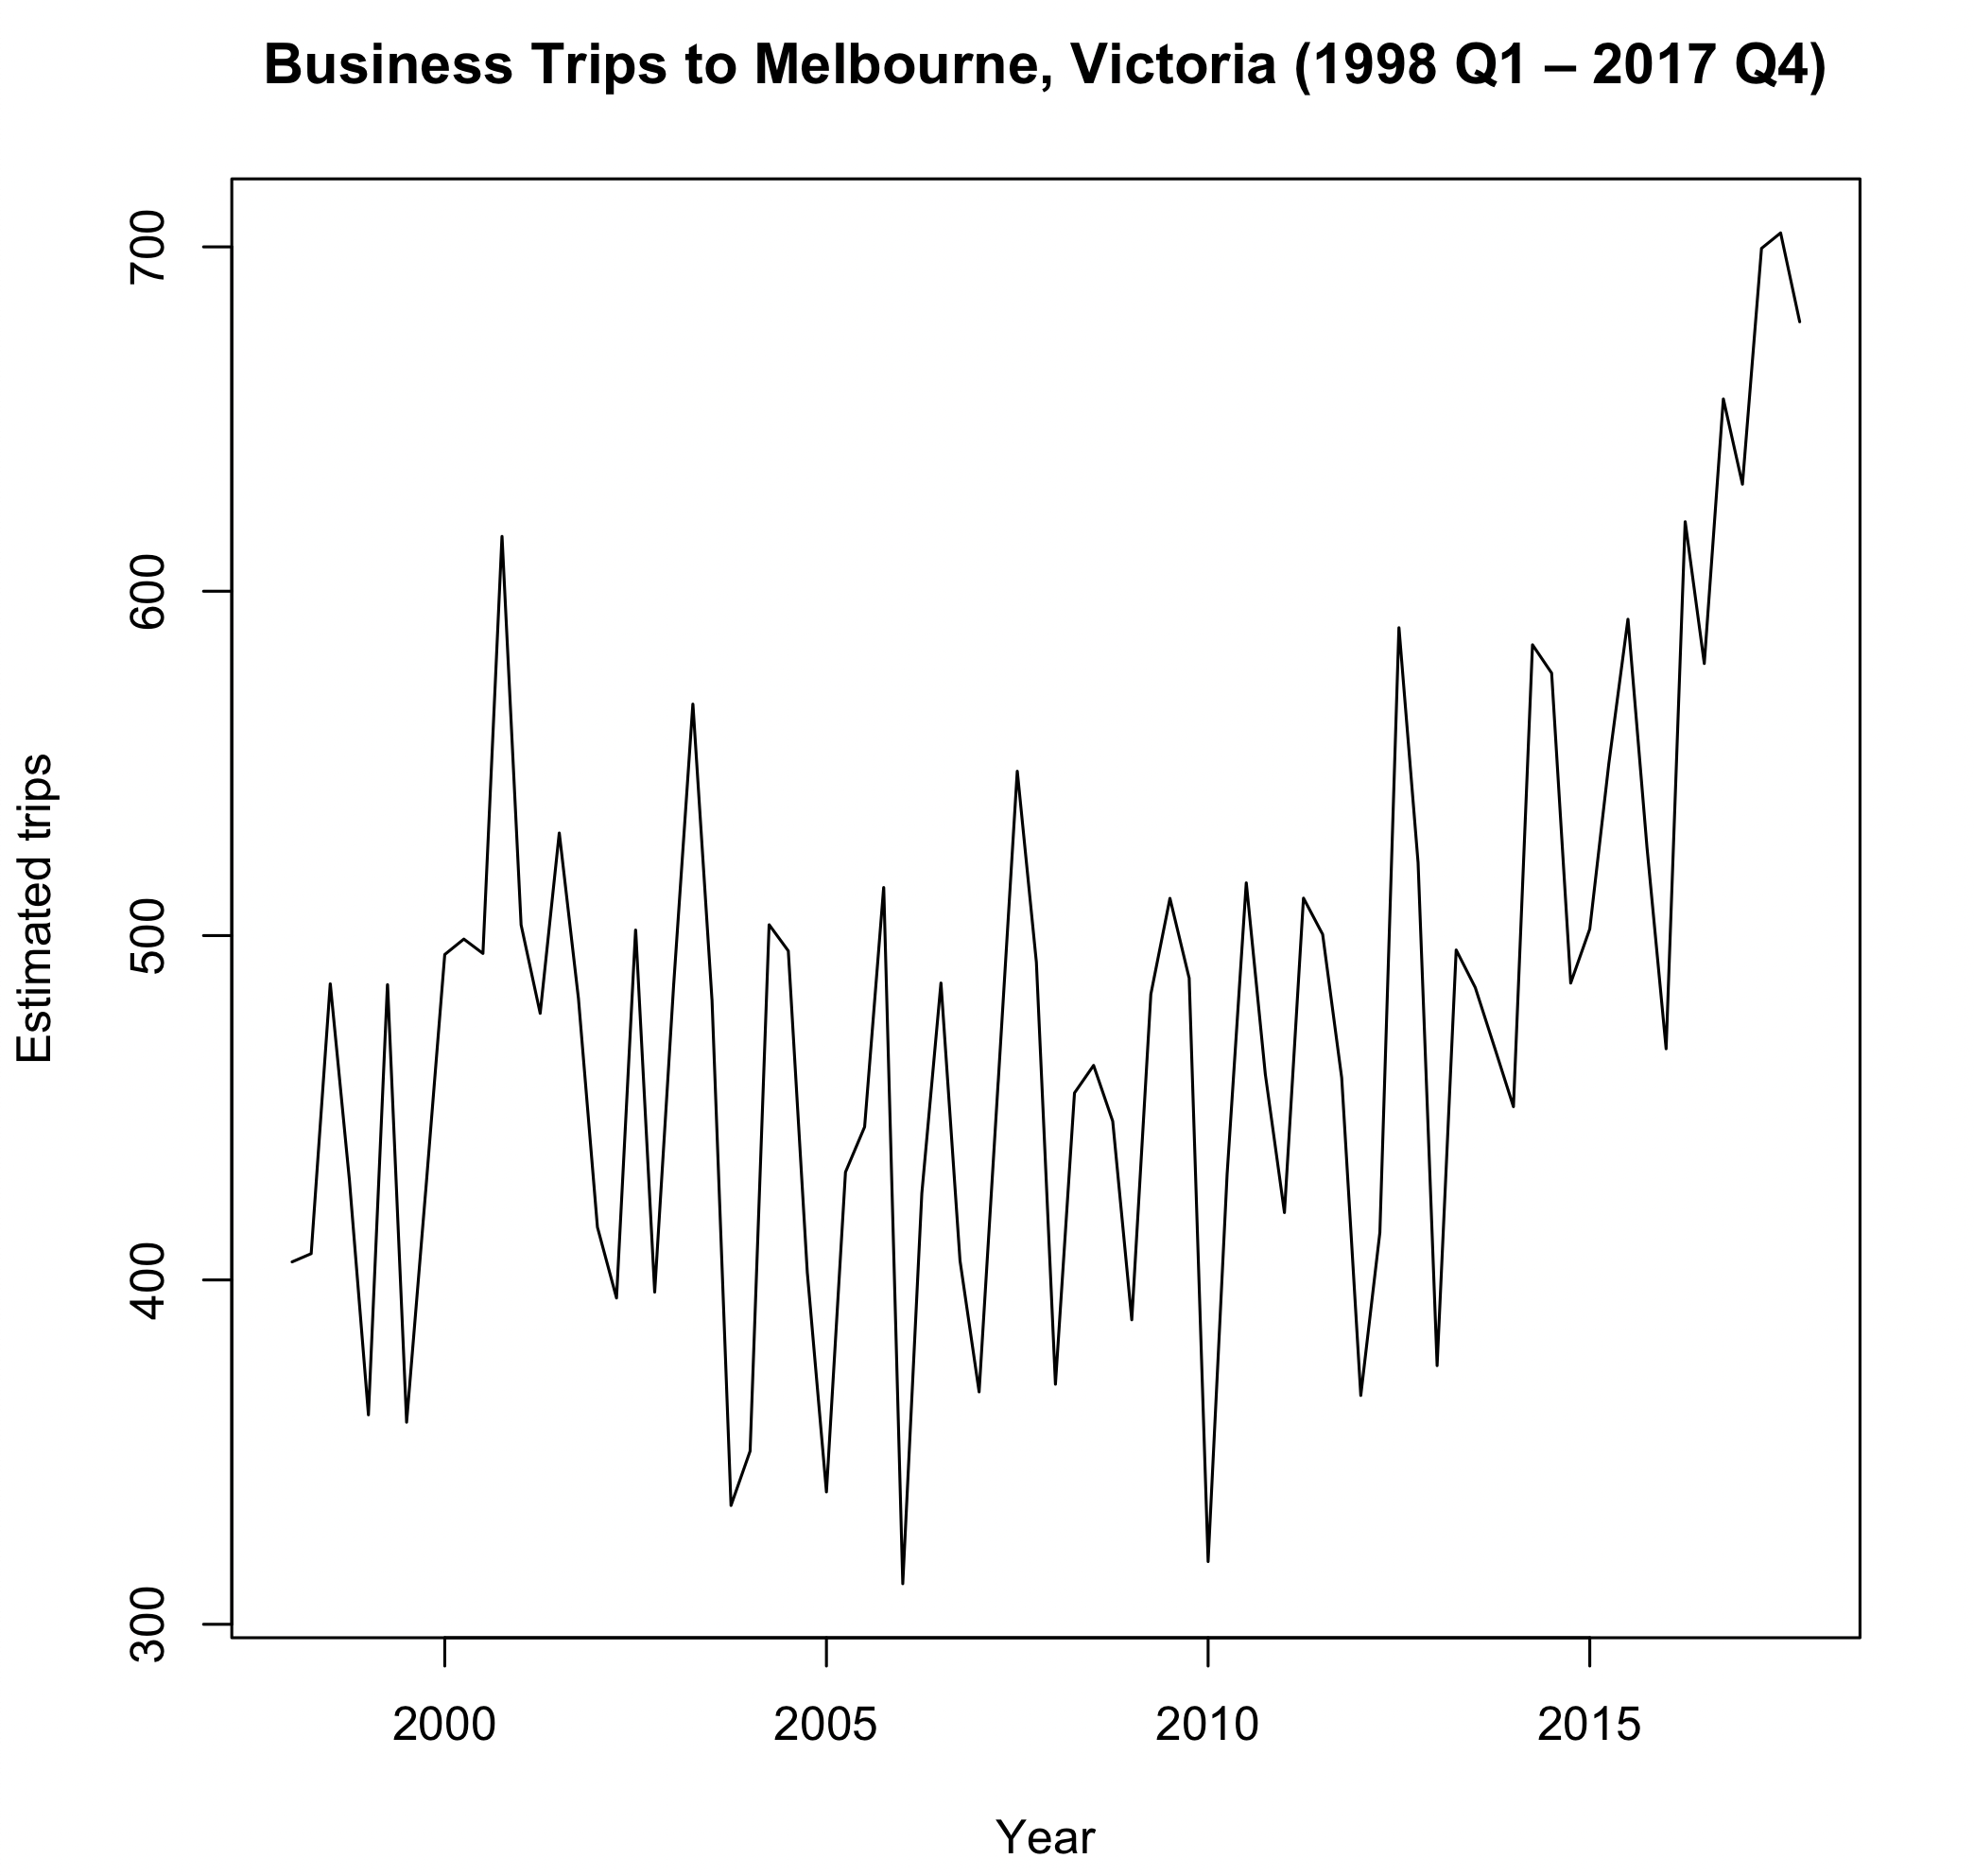
\includegraphics[width=0.55\linewidth]{fig/y1timeplot.png}
\end{figure}

\noindent The time plot exhibits two distinct phases. From 1998 to around 2010, the series fluctuates without a clear trend. From 2010 onwards, it shows a strong upward trend, accelerating after 2014 and reaching a peak of approximately 700 trips in 2017. A clear annual seasonal pattern is also evident throughout the period. Overall, the average number of Business trips increased from about 400 in 1998 to 700 in 2017, representing an increase of approximately 57\%.
% \begin{lstlisting}[language=R]
% layout(1:2)
% plot(aggregate(y1))
% \end{lstlisting}

\begin{figure}[H]
    \centering
    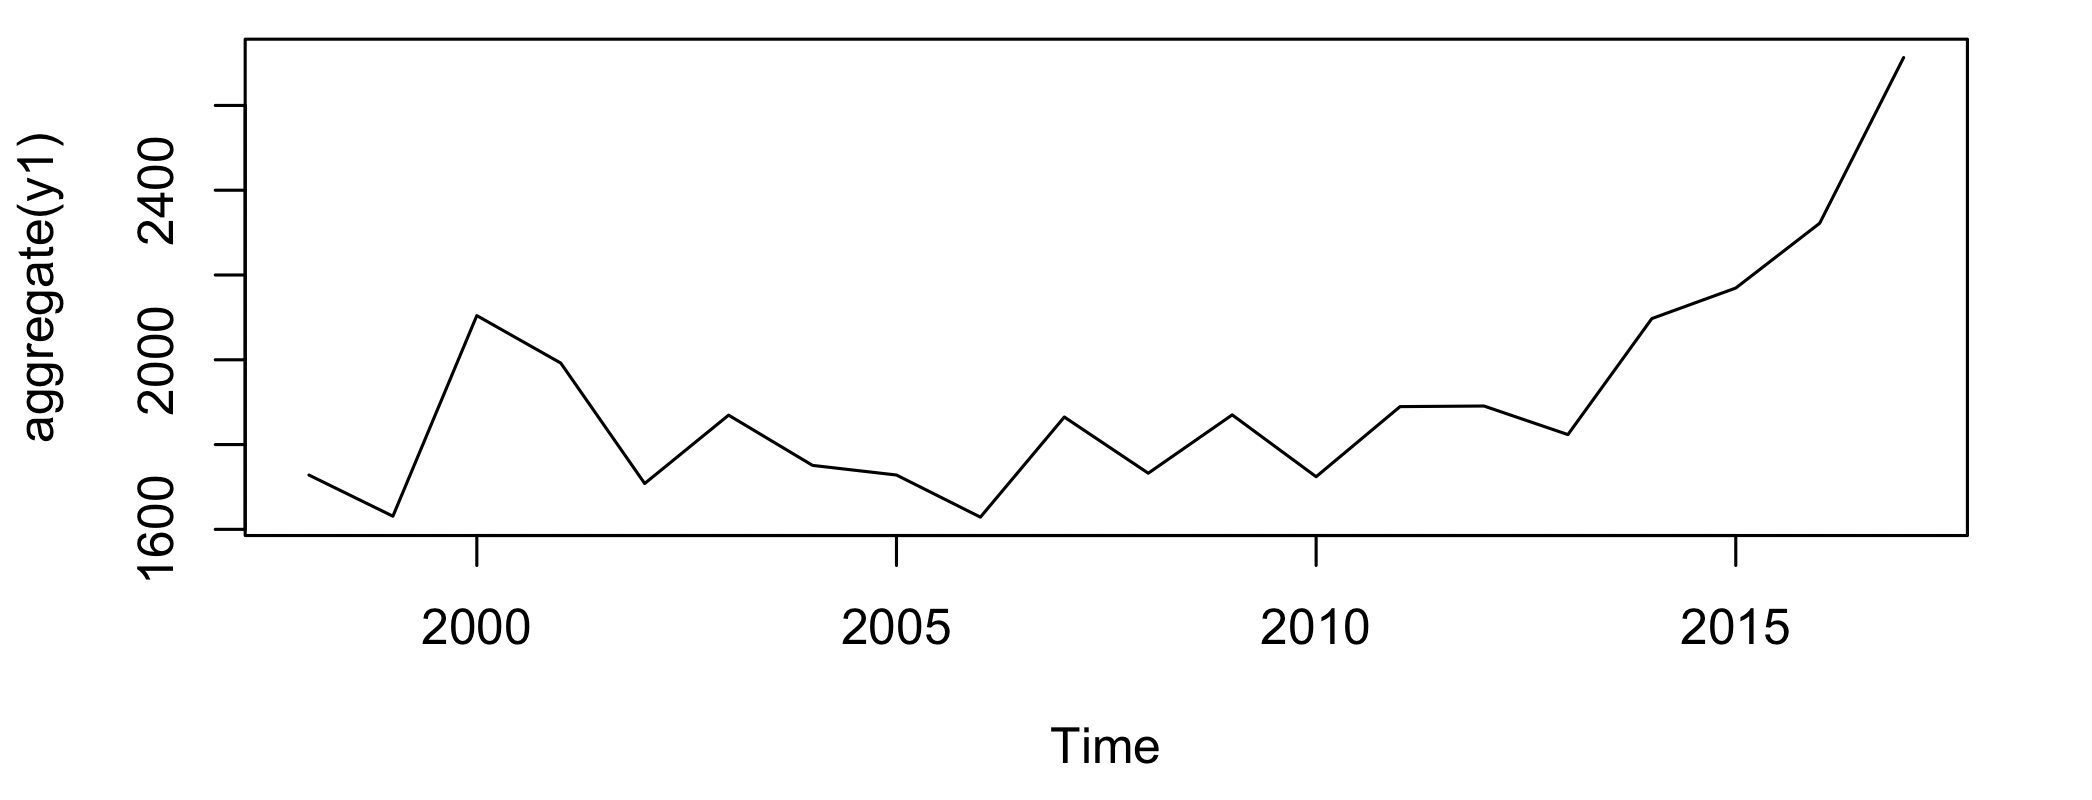
\includegraphics[width=0.65\linewidth]{fig/y1aggregate.png}
\end{figure}
\noindent To get a clearer view of the trend, the seasonal effect can be removed by aggregating the data to annual level.
\noindent It is apparent from the annual series that the number of business trips to Melbourne is increasing over time. The annual total is approximately 1728 trips in 1998, reaching a total of approximately 2713 trips by 2017. Aligned with our previous observations, the plot does not show any clear directional movement from around 2002 to 2010, and continues with a clear and continuous upward trend afterwards.
\pagebreak
\noindent Additionally, with the boxplot of the series, we can further see the seasonal effects.\\

% \begin{lstlisting}[language=R]
% boxplot(y1 ~ cycle(y1),
% 		names = c("Q1","Q2","Q3","Q4"),
% 		main = "Seasonal boxplot of Business Trips",
% 		xlab = "Quarter", ylab = "Number of Trips")
% \end{lstlisting}

\begin{figure}[H]
    \centering
    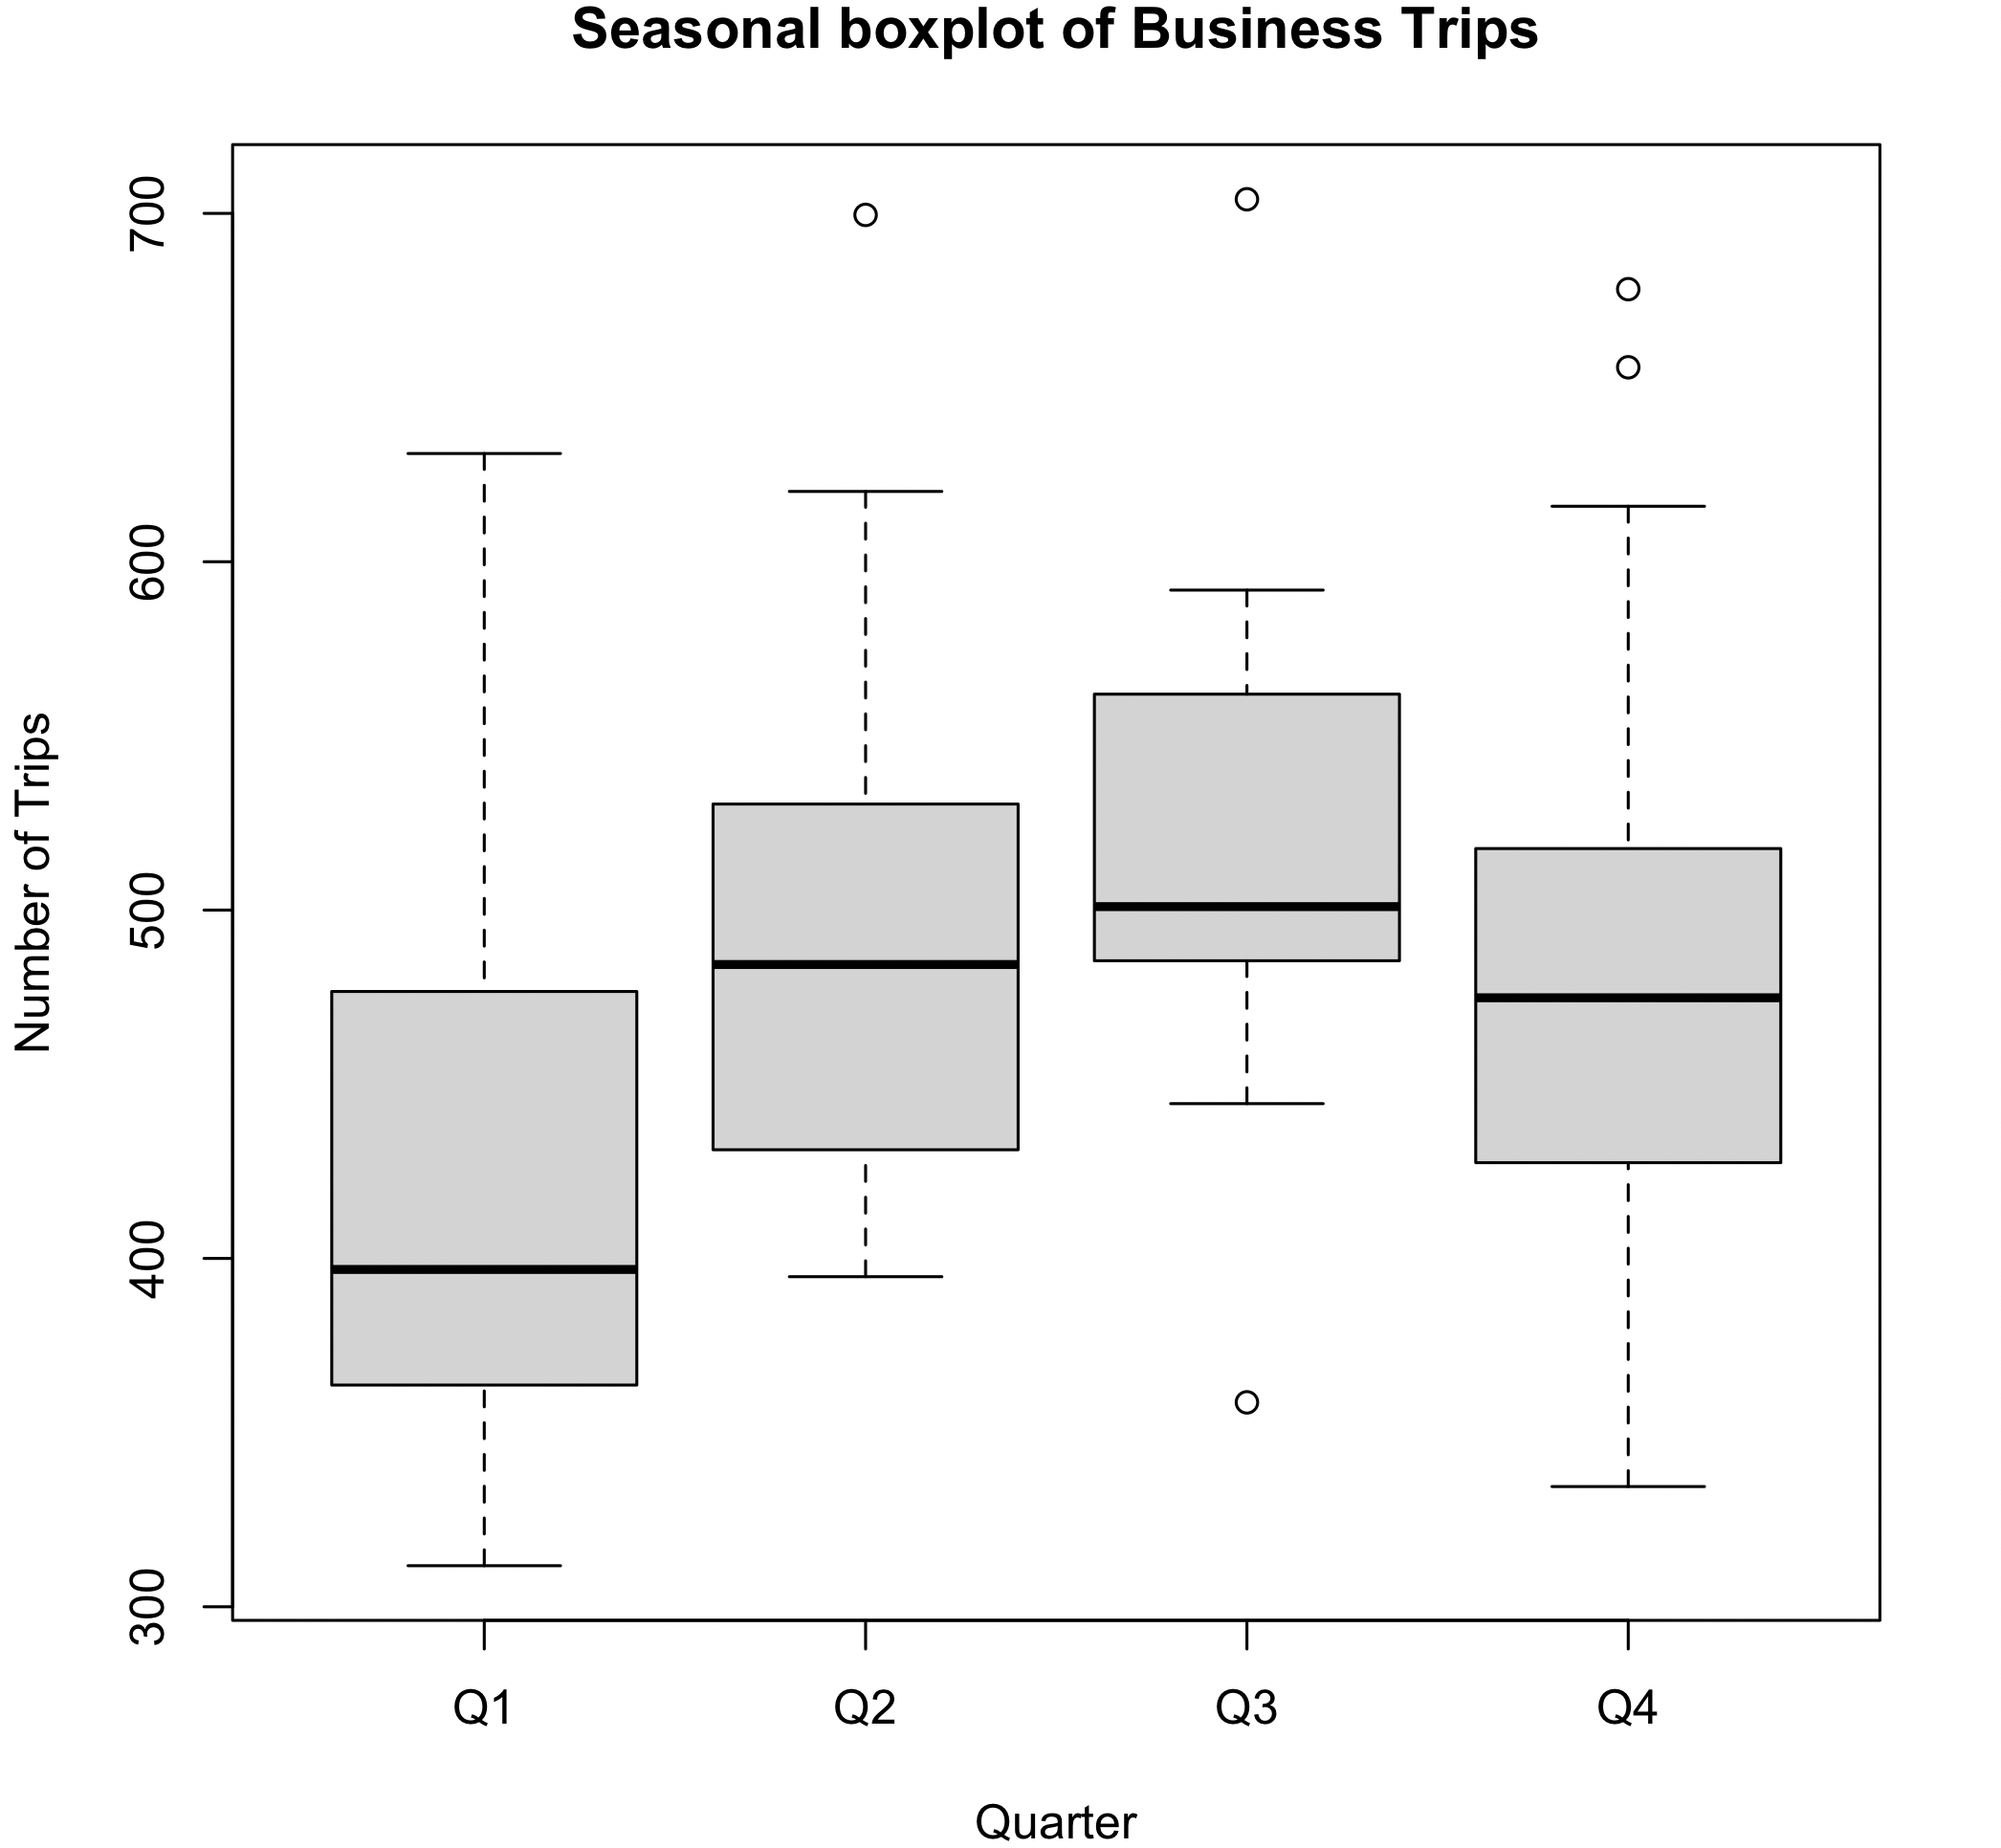
\includegraphics[width=0.55\linewidth]{fig/y1boxplot.png}
\end{figure}

\noindent Trip bookings are highest during July to September with an average of approximately 500 trips, and lowest during January to March with an average of approximately 400 trips. Q2 and Q4 falls in between, averaging approximately 490 trips. The differences across quarters are apparent, confirming that business travels to Melbourne is strongly dependent on the time of year.\\
\noindent A possible explanation for this seasonal pattern, is that business activities tend to be higher in the middle of the year.

\subsection{Holiday Series}
\begin{figure}[h]
    \centering
    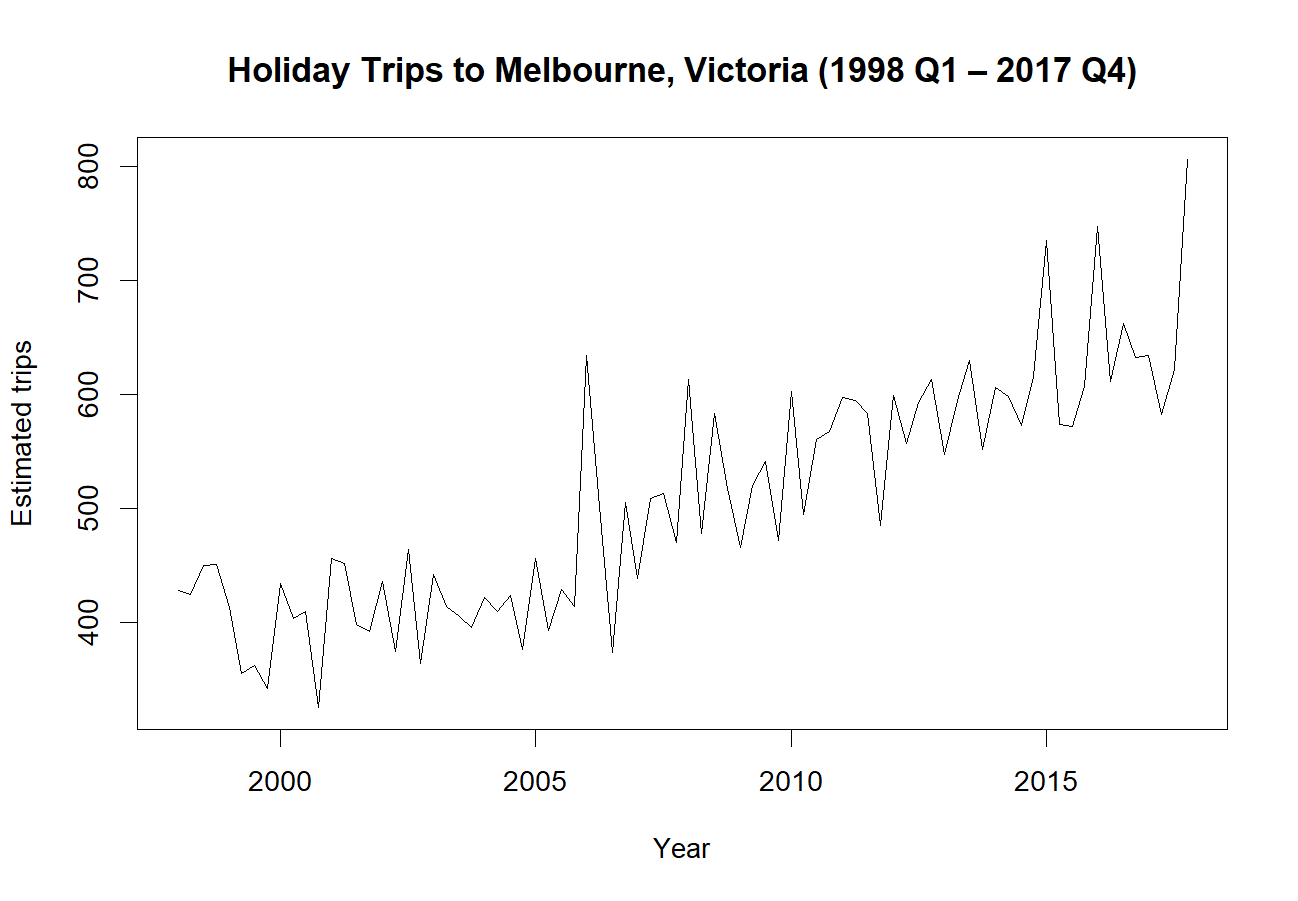
\includegraphics[width=0.55\linewidth]{fig/figy2timeplot.png}
\end{figure}

\noindent The time plot shows that different phases over the observation period. From 1998 to around 2005, the series fluctuates around a relatively stable level without a clear trend. From 2006 onwards, it shows an upward trend, which becomes more pronounced after 2010, reaching a peak of approximately 800 trips in 2017. A clear annual seasonal pattern is also evident throughout the period. Overall, the average number of Holiday trips increased from about 400 in 1998 to 800 in 2017, representing an increase of approximately 100\%.

\begin{figure}[h]
    \centering
    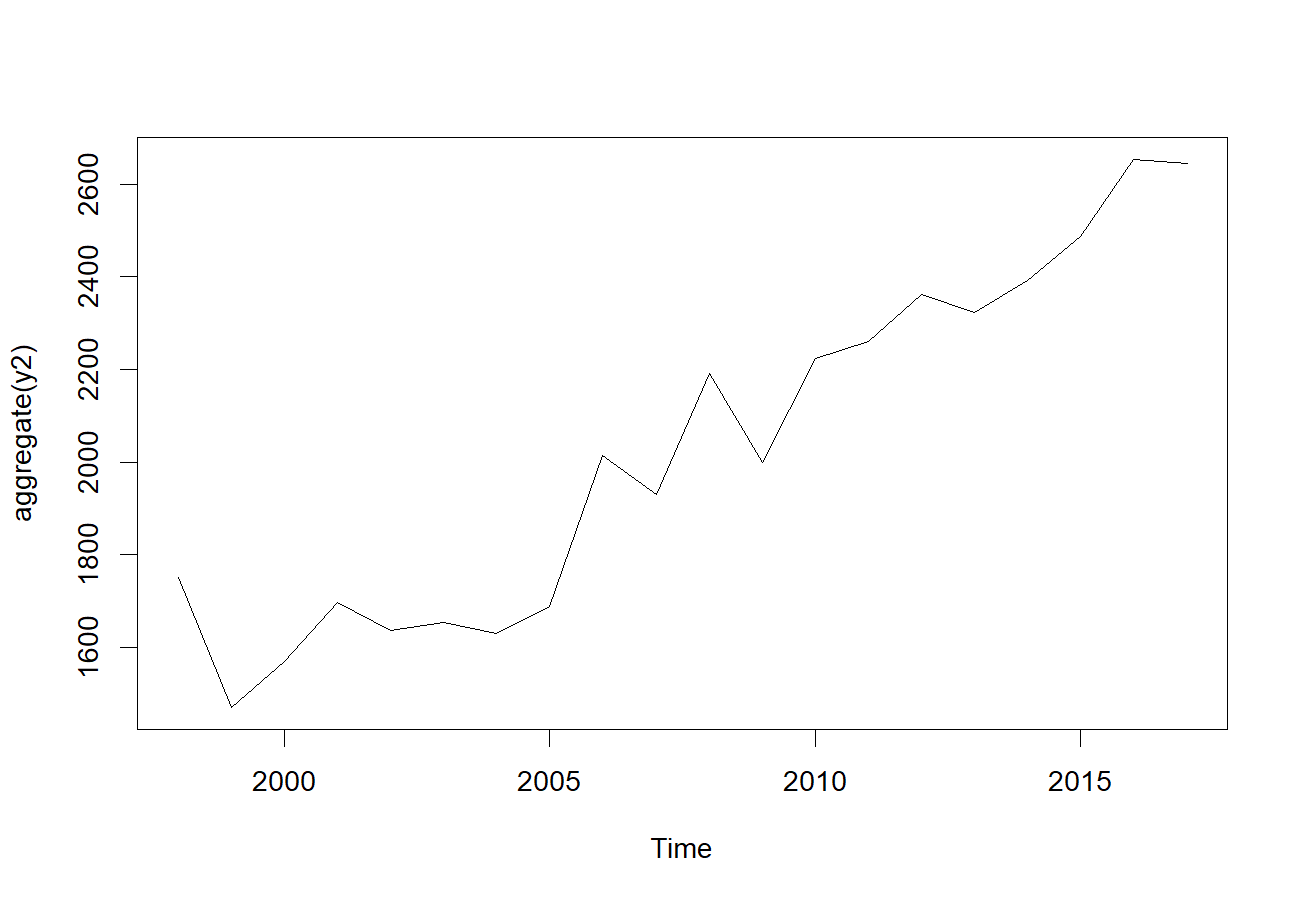
\includegraphics[width=0.65\linewidth]{fig/y2aggregate.png}
\end{figure}

\noindent To obtain a clearer view of the long-term trend, the seasonal effect can be reduced by aggregating the quarterly data into annual observations.
\noindent The aggregate plot confirms the overall increasing trend observed in the Holiday series. From 1998 to around 2005, the annual number of holiday trips remains relatively stable, fluctuating between approximately 1,500 and 1,700 trips. From 2006 onwards, the series exhibits a clear upward trend, although there are slight year-to-year fluctuations. The annual number of holiday trips increases steadily and reaches approximately 2,650 trips towards the end of the observation period, indicating sustained growth in holiday travel to Melbourne.
\noindent Thus, the quarterly boxplot of the series provides further evidence of seasonal variation.
\begin{figure}[h]
    \centering    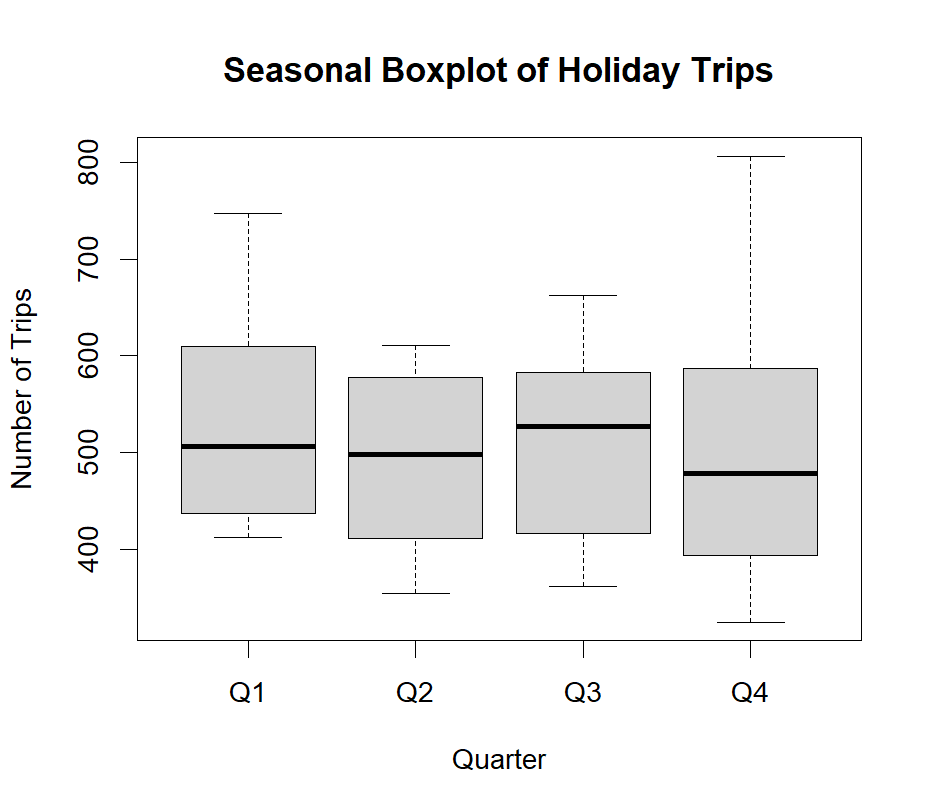
\includegraphics[width=0.55\linewidth]{fig/y2boxplot.png}
\end{figure}

\noindent The seasonal boxplot shows that the number of holiday trips varies across the four quarters. Quarter 3 has the highest median, at around 525 trips, while Quarter 4 has the lowest median, at around 480 trips. Quarter 1 and Quarter 2 fall in between, with median values of about 505 and 500 trips. Quarter 4 also shows a wider spread than the other quarters, meaning that the number of holiday trips is more variable during this quarter. Although the differences are not very large, they still suggest that holiday trips follow a seasonal pattern.\\
\noindent A possible explanation for this seasonal pattern is that holiday travel demand changes throughout the year due to factors such as school holidays and public holidays.

\subsection{Conclusion of the Two Series}

\noindent In conclusion, both Business and Holiday series show an increasing trend and clear quarterly seasonal patterns over the observation period. The Holiday series demonstrates a stronger growth trend compared to the Business series, while both series exhibit variations across different quarters. Therefore, trend and seasonal components should be considered when fitting appropriate time series models.

% Time Series Decomposition
\section{Time Series Decomposition}
\subsection{Business Series}
Both additive and multiplicativedecomposition models were applied to the Business series. In the additive model, the observed series is expressed as:
\[x_t = m_t + s_t + z_t\]
where $m_t$ is the trend, $s_t$ is the seasonal effect, and $z_t$ is the random component with mean zero. In the multiplicative model, the series is expressed as:
$x_t = m_t  \cdot s_t \cdot z_t$
where the seasonal effect is assumed to grow in proportion to the trend.
To determine which model is more appropriate, both decompositions were plotted and the random components were compared. 
% \begin{lstlisting}[language=R]
% decom1.add <- decompose(y1)
% decom1.mul <- decompose (y1, type="mult")

% plot(decom1.add)
% plot(decom1.mul)
% \end{lstlisting}
\begin{figure}[ht]
    \centering
    \begin{minipage}{0.49\textwidth}
        \centering
        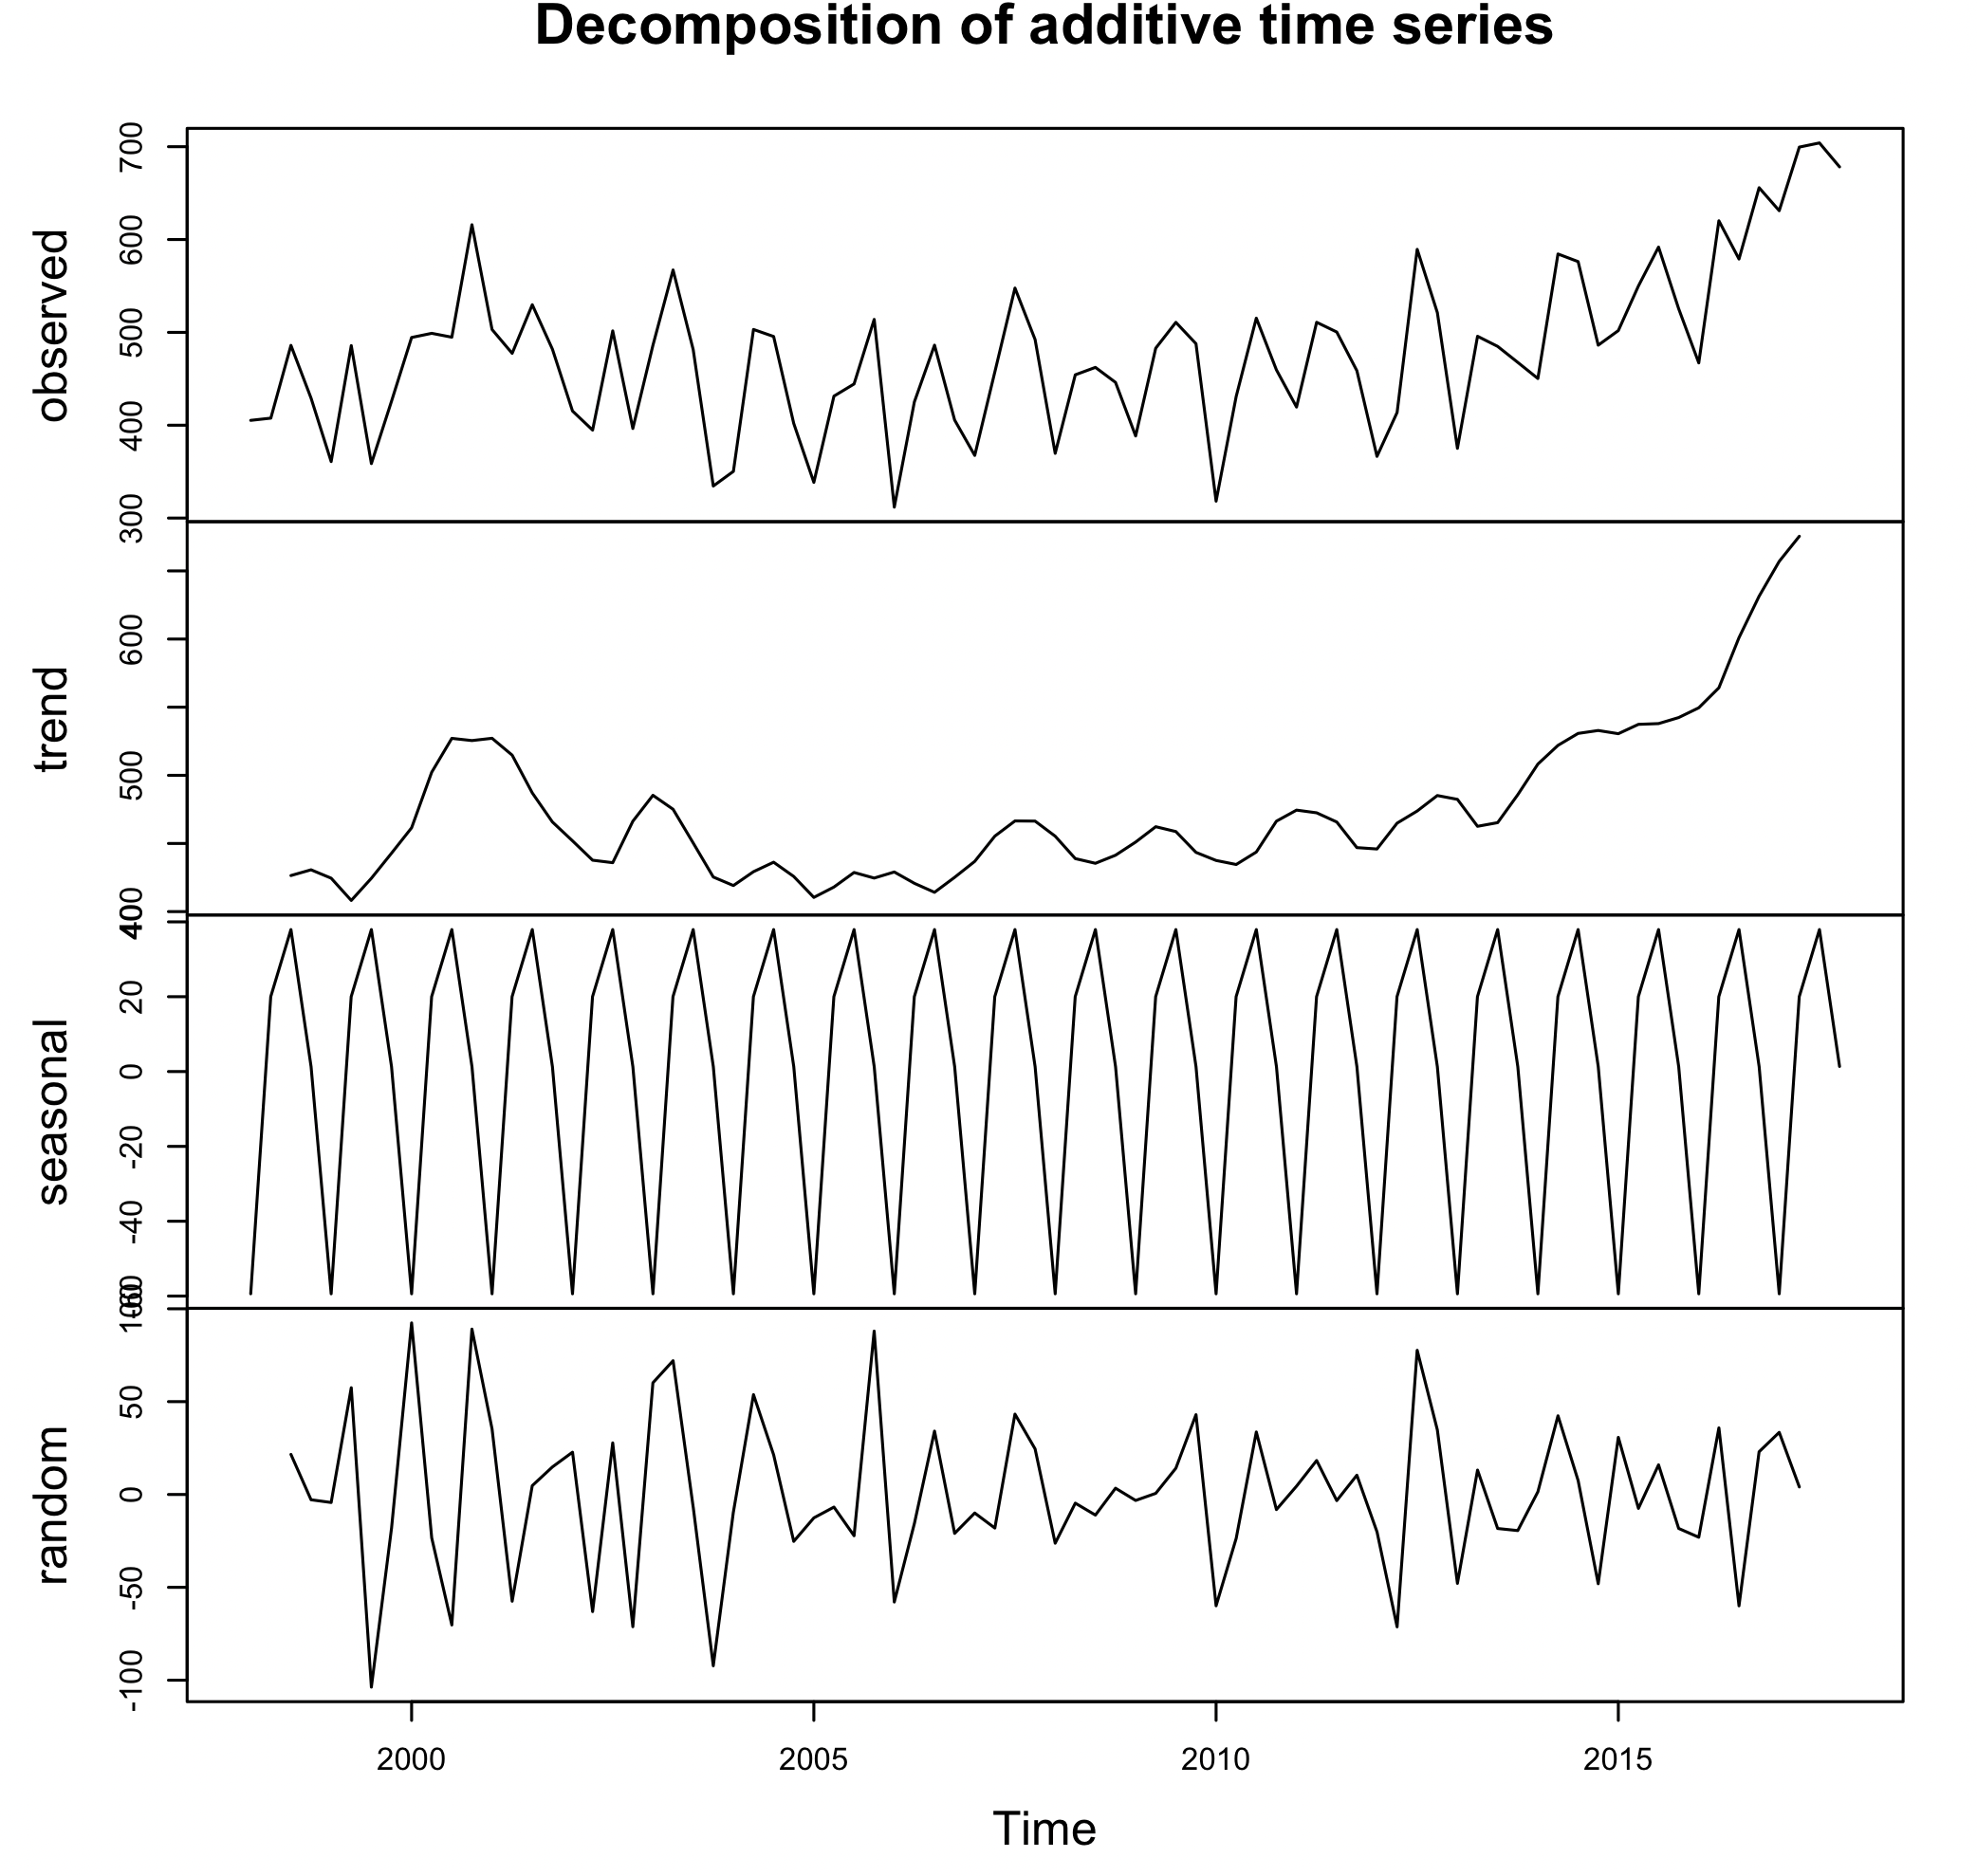
\includegraphics[width=1\linewidth]{fig/y1add.png}
        \caption{Additive decomposition}
        \label{fig:y1add}
    \end{minipage}
    \hfill
    \begin{minipage}{0.49\textwidth}
        \centering
        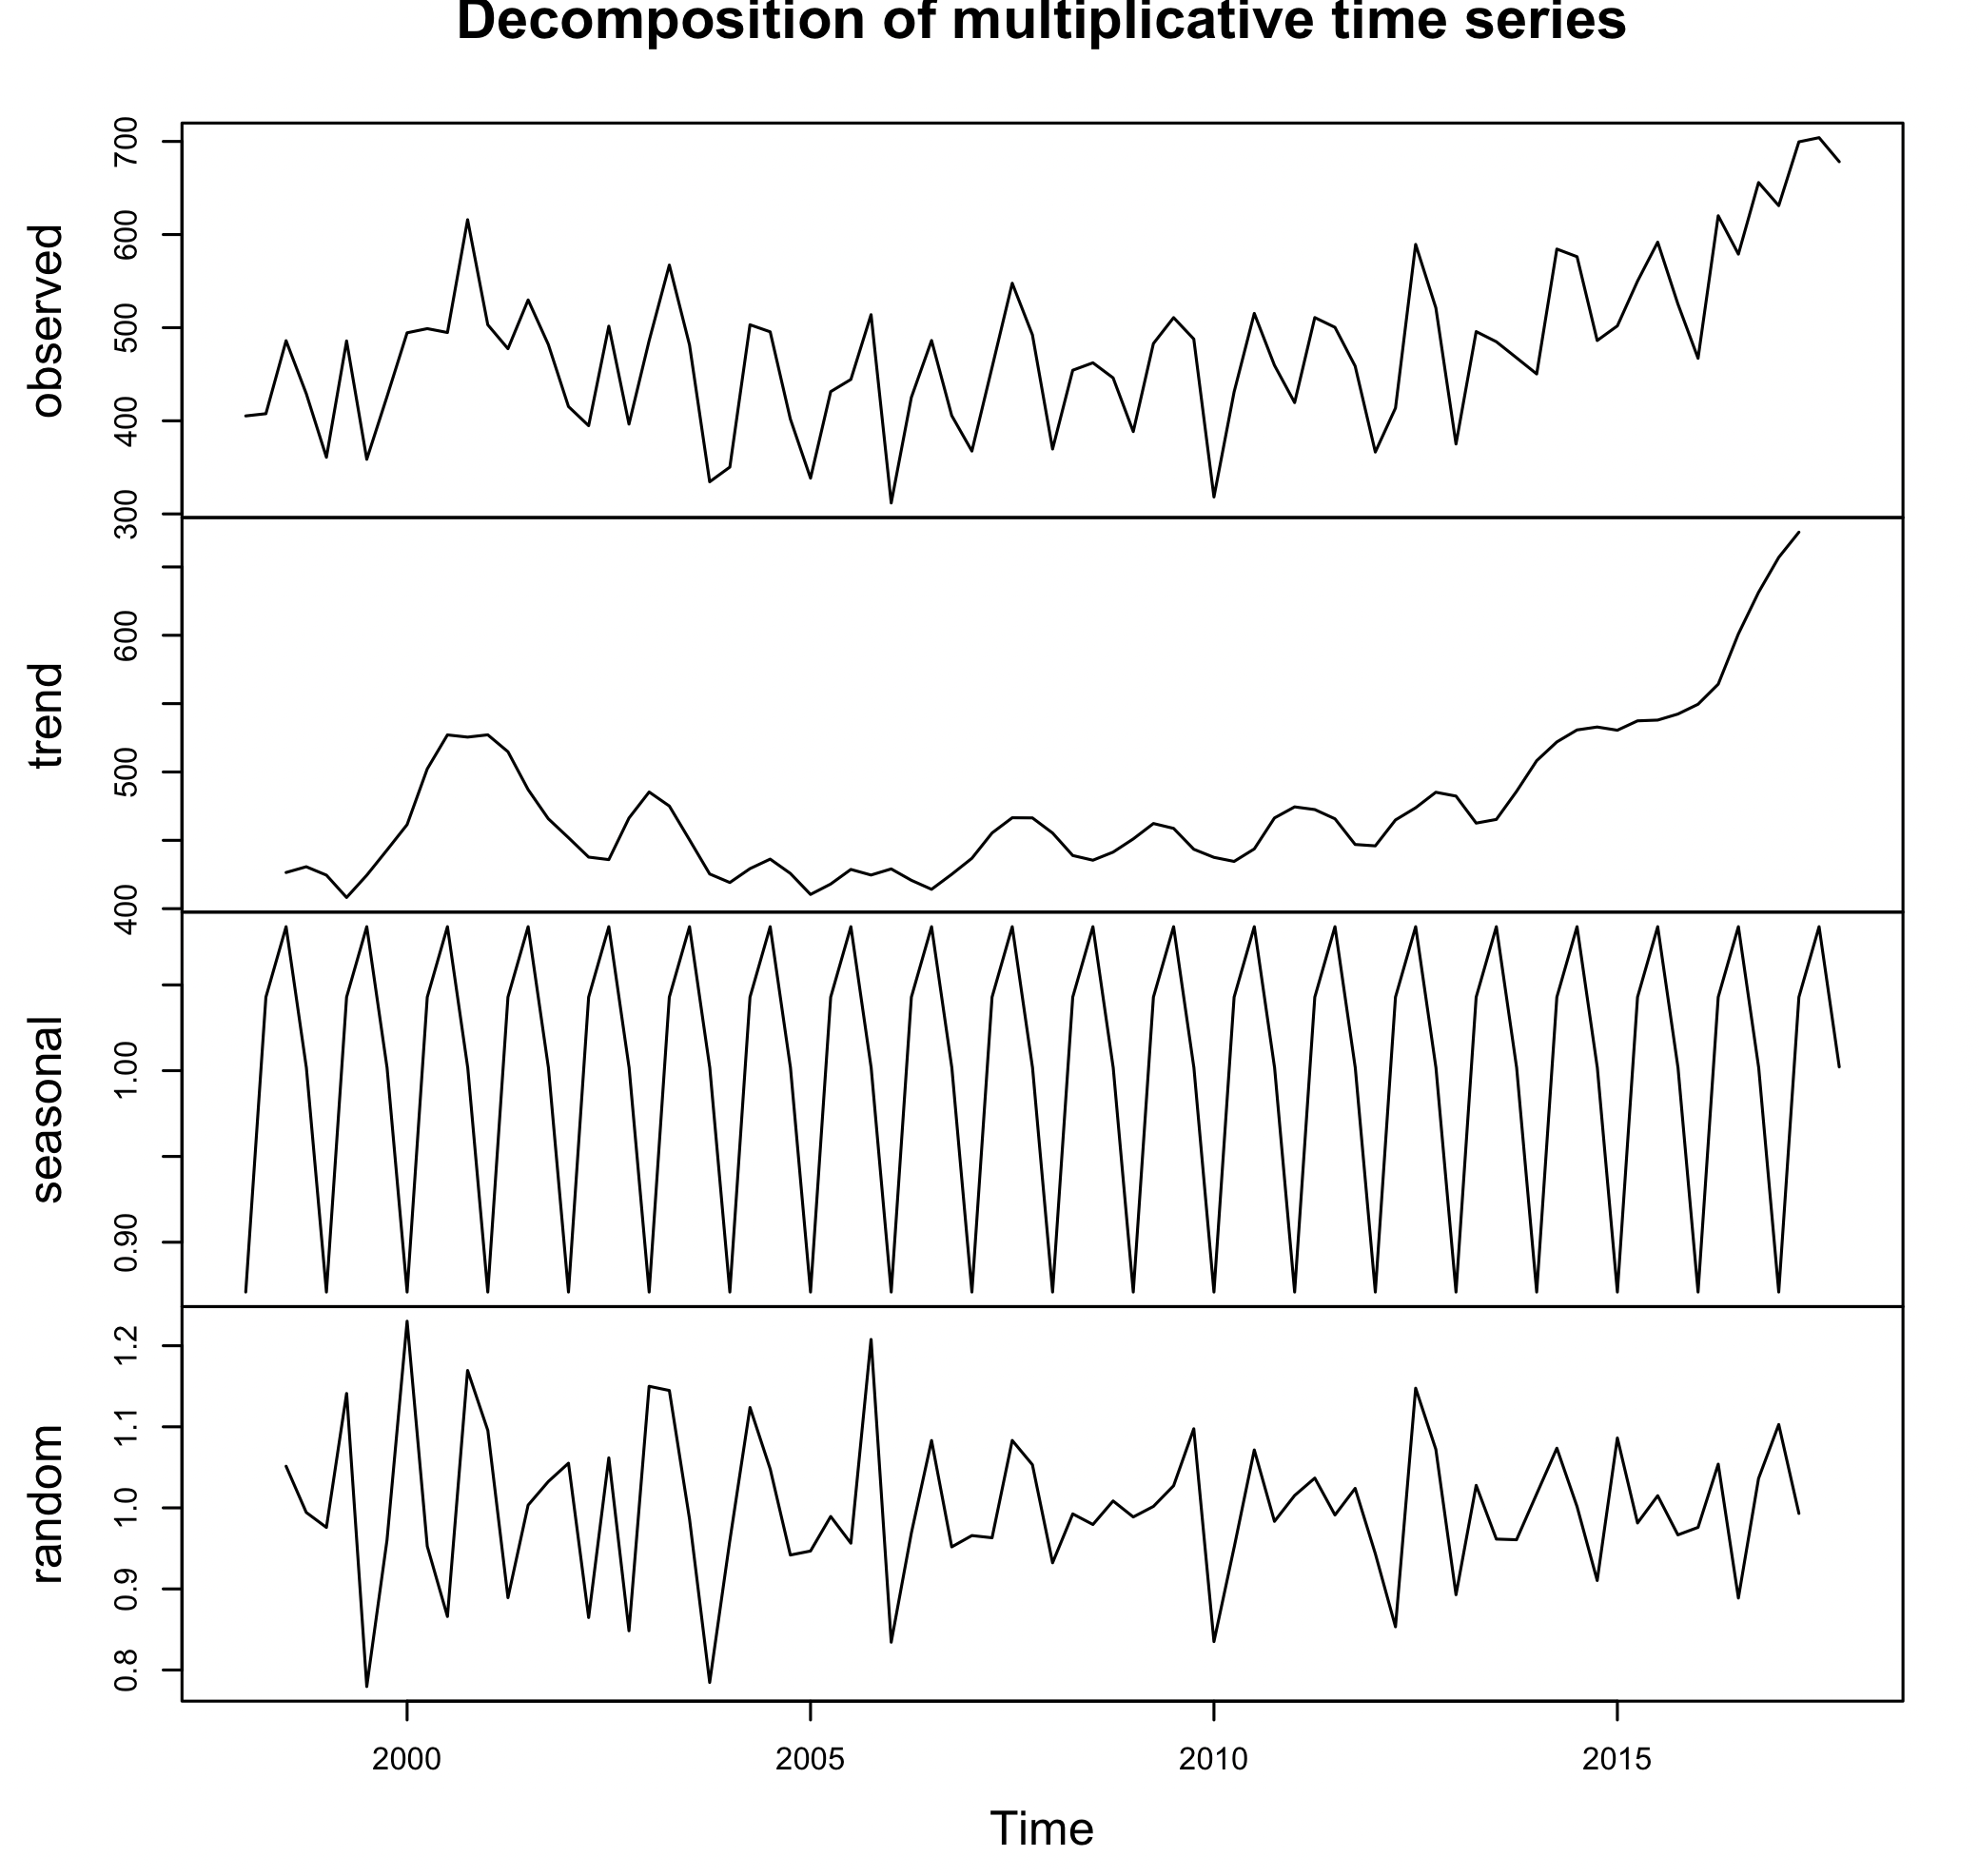
\includegraphics[width=1\linewidth]{fig/y1mul.png}
        \caption{Multiplicative decomposition}
        \label{fig:y1mul}
    \end{minipage}
\end{figure}

\noindent For the Business series, the seasonal variation does not appear to increase as the trend increases, the size of the seasonal swings remains roughly constant across the full observation period. Comparing the random components of the two models, the multiplicative residuals seems slightly more uniform as the are centered around 1.\\

\noindent Therefore we conclude that the additive decomposition model is more appropriate for the Business series, with the features:
\begin{enumerate}
    \item The trend component confirms the 2-phase behavior we observed in the time plot.
    \item The seasonal component shows a consistent repeating pattern, which is stable throughout the whole observation period.
    \item The random component shows no systematic pattern in size over time.
\end{enumerate}

\subsection{Holiday Series}

\noindent Both additive and multiplicative decomposition models were applied to the Holiday series. 
In the additive model, the observed series is expressed as:
\[
x_t = m_t + s_t + z_t
\]
where \(m_t\) represents the trend component, \(s_t\) represents the seasonal component, 
and \(z_t\) represents the random component with mean zero. 

\noindent In the multiplicative model, the series is expressed as : \[
x_t = m_t \cdot s_t \cdot z_t
\]where the seasonal variation is assumed to change proportionally with the trend.

\begin{figure}[ht]
    \centering
    \begin{minipage}{0.49\textwidth}
        \centering
        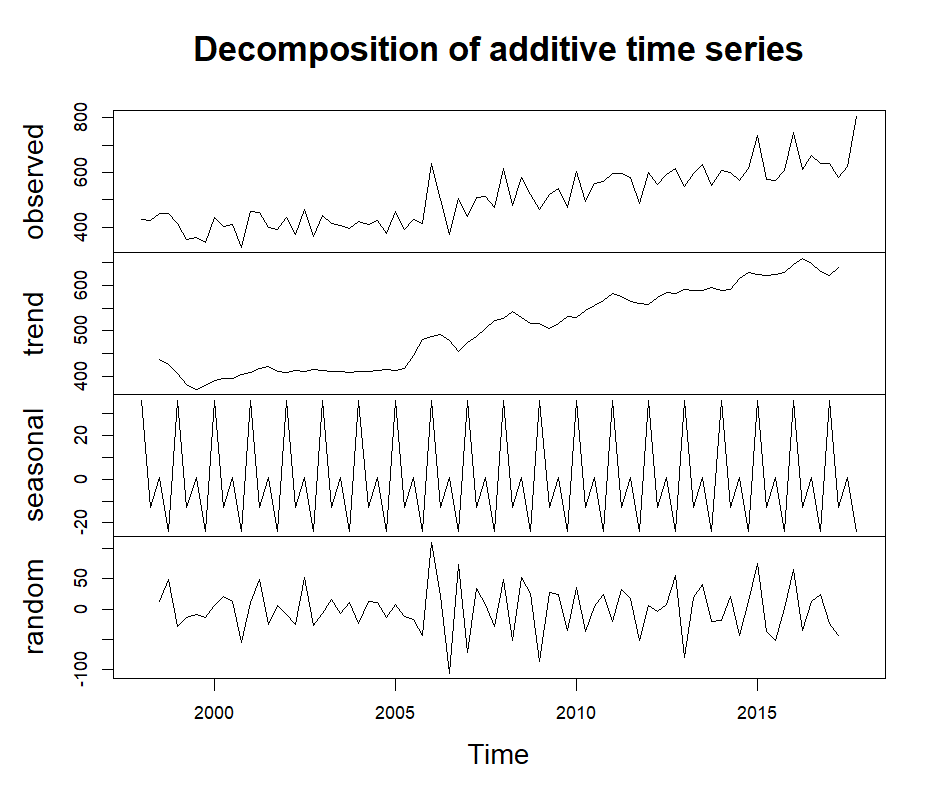
\includegraphics[width=1\linewidth]{fig/y2add.png}
            \caption{Additive decomposition}
        \label{fig:y2add}
    \end{minipage}
    \hfill
    \begin{minipage}{0.49\textwidth}
        \centering
        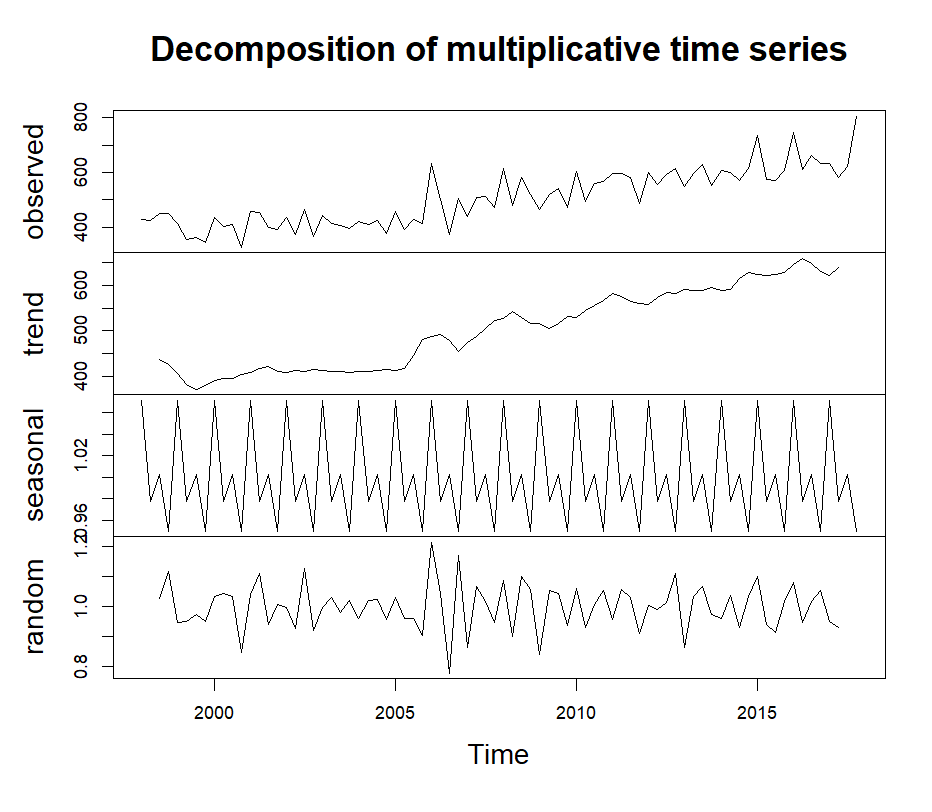
\includegraphics[width=1\linewidth]{fig/y2mul.png}
        \caption{Multiplicative decomposition}
        \label{fig:y2mul}
    \end{minipage}
\end{figure}


\noindent Figures 3 and 4 show that the additive and multiplicative decomposition results of the Holiday series. Both decomposition methods indicate the presence of trend and seasonal components. The trend component shows an overall increasing pattern, with a more noticeable increase after approximately 2006. The seasonal component exhibits a clear and consistent quarterly pattern throughout the observation period.

\noindent The seasonal variation appears to increase as the trend increases, and the size of the seasonal fluctuates over the entire observation period. Therefore, the multiplicative decomposition model is considered more appropriate for the Holiday series. The additive decomposition is included for comparison.

% Correlation Structure
\section{Correlation Structure}
\subsection{Business Series}
% \begin{lstlisting}[language=R]
% layout(1:2)
% acf(y1, main="Business Series")
% \end{lstlisting}
\vspace{-0.4cm}
\begin{figure}[H]
    \centering
    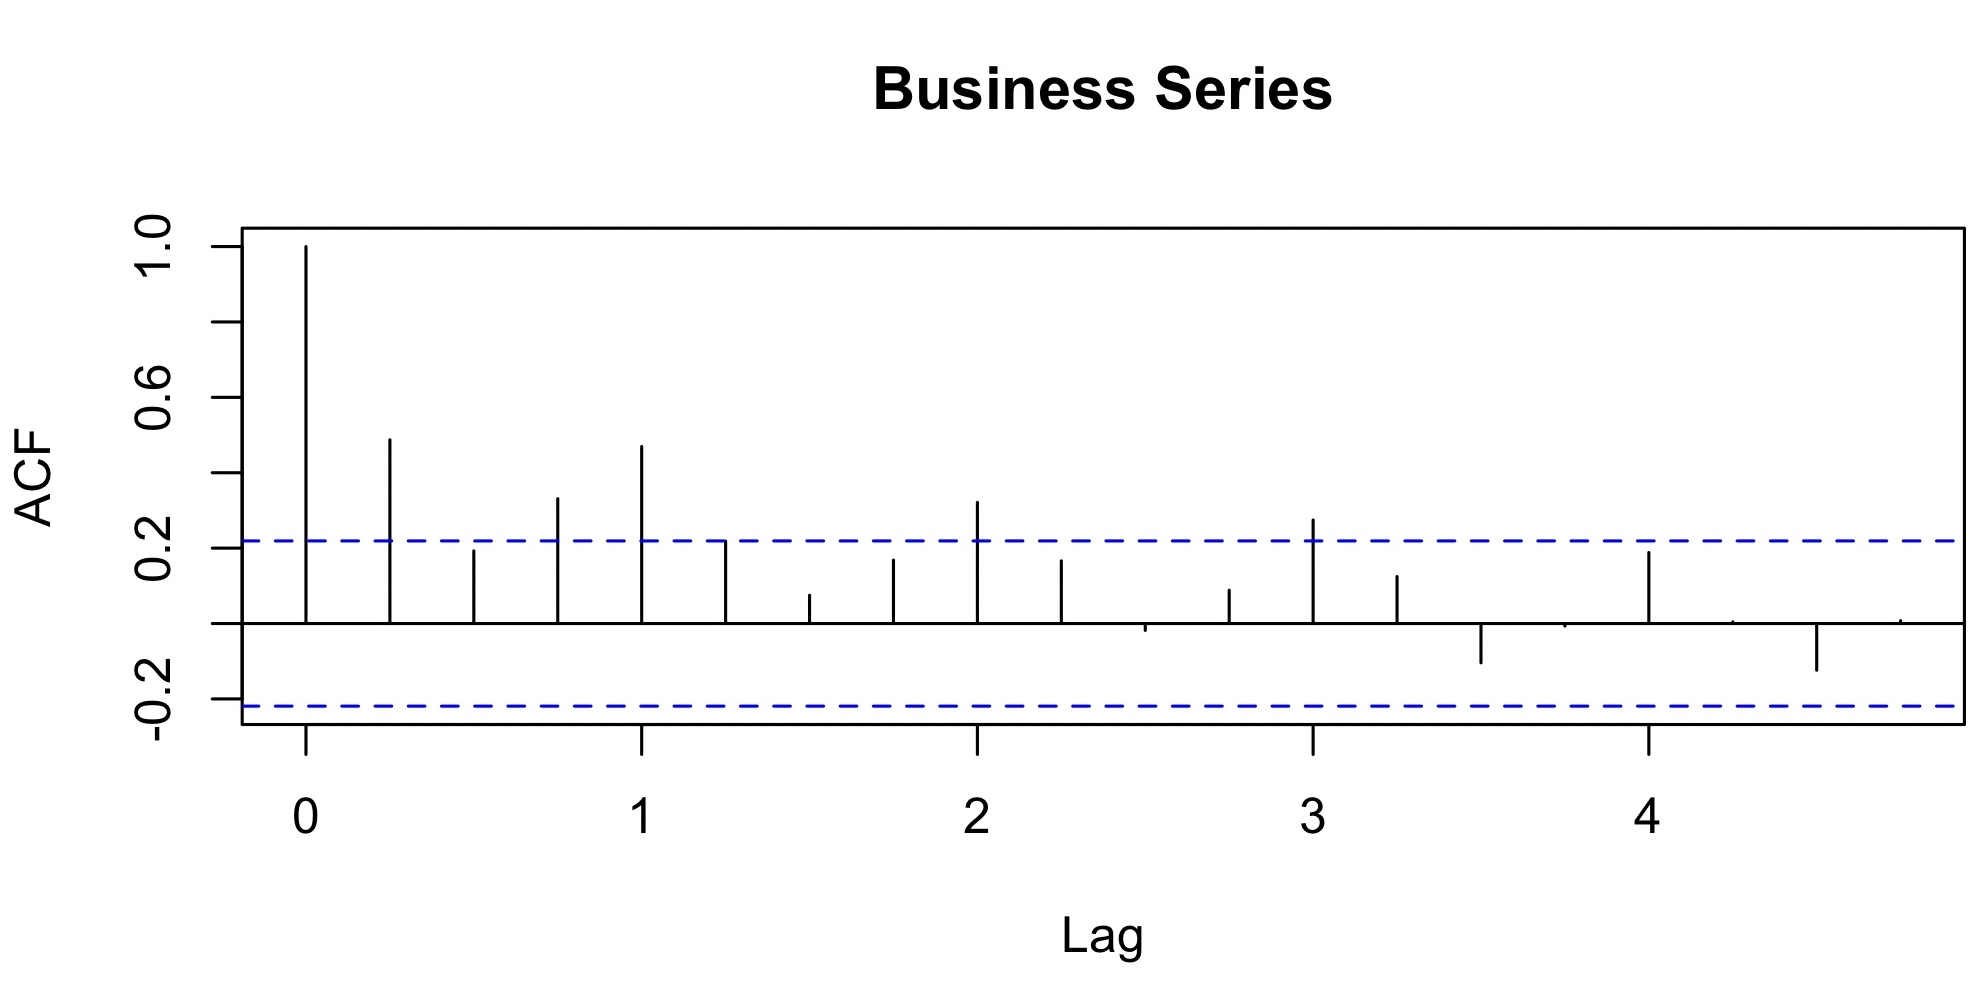
\includegraphics[width=0.65\linewidth]{fig/y1acf.jpg}
\end{figure}
\vspace{-0.4cm}
\noindent The correlogram does not decay to zero within a few lags, suggesting that the business series is unlikely to be stationary. The autocorrelations rise and fall in a repeating pattern, with peaks at lags 4, 8 and 12, reflecting a strong positive autocorrelation between pairs of quarters separated by multiples of four. That is, the same quarter in different years. This suggests a seasonal variation in the series. The autocorrelation at lag 1 is also large and positive, exceeding the dashed 95\% reference lines, so that business trips in one quarter are also correlated with trips in the following quarter. The physical interpretation is that a business quarter with above-average trips tends to be followed by a further above-average quarter. This suggests that the number of business trips in a given quarter tends to resemble that of the corresponding quarter in the following year. This behaviour is typical of a series with unremoved seasonal variation.
\vspace{0.4cm}
% \begin{lstlisting}[language=R]
% pacf(y1, main="Business Series")
% \end{lstlisting}
\begin{figure}[H]
    \centering
    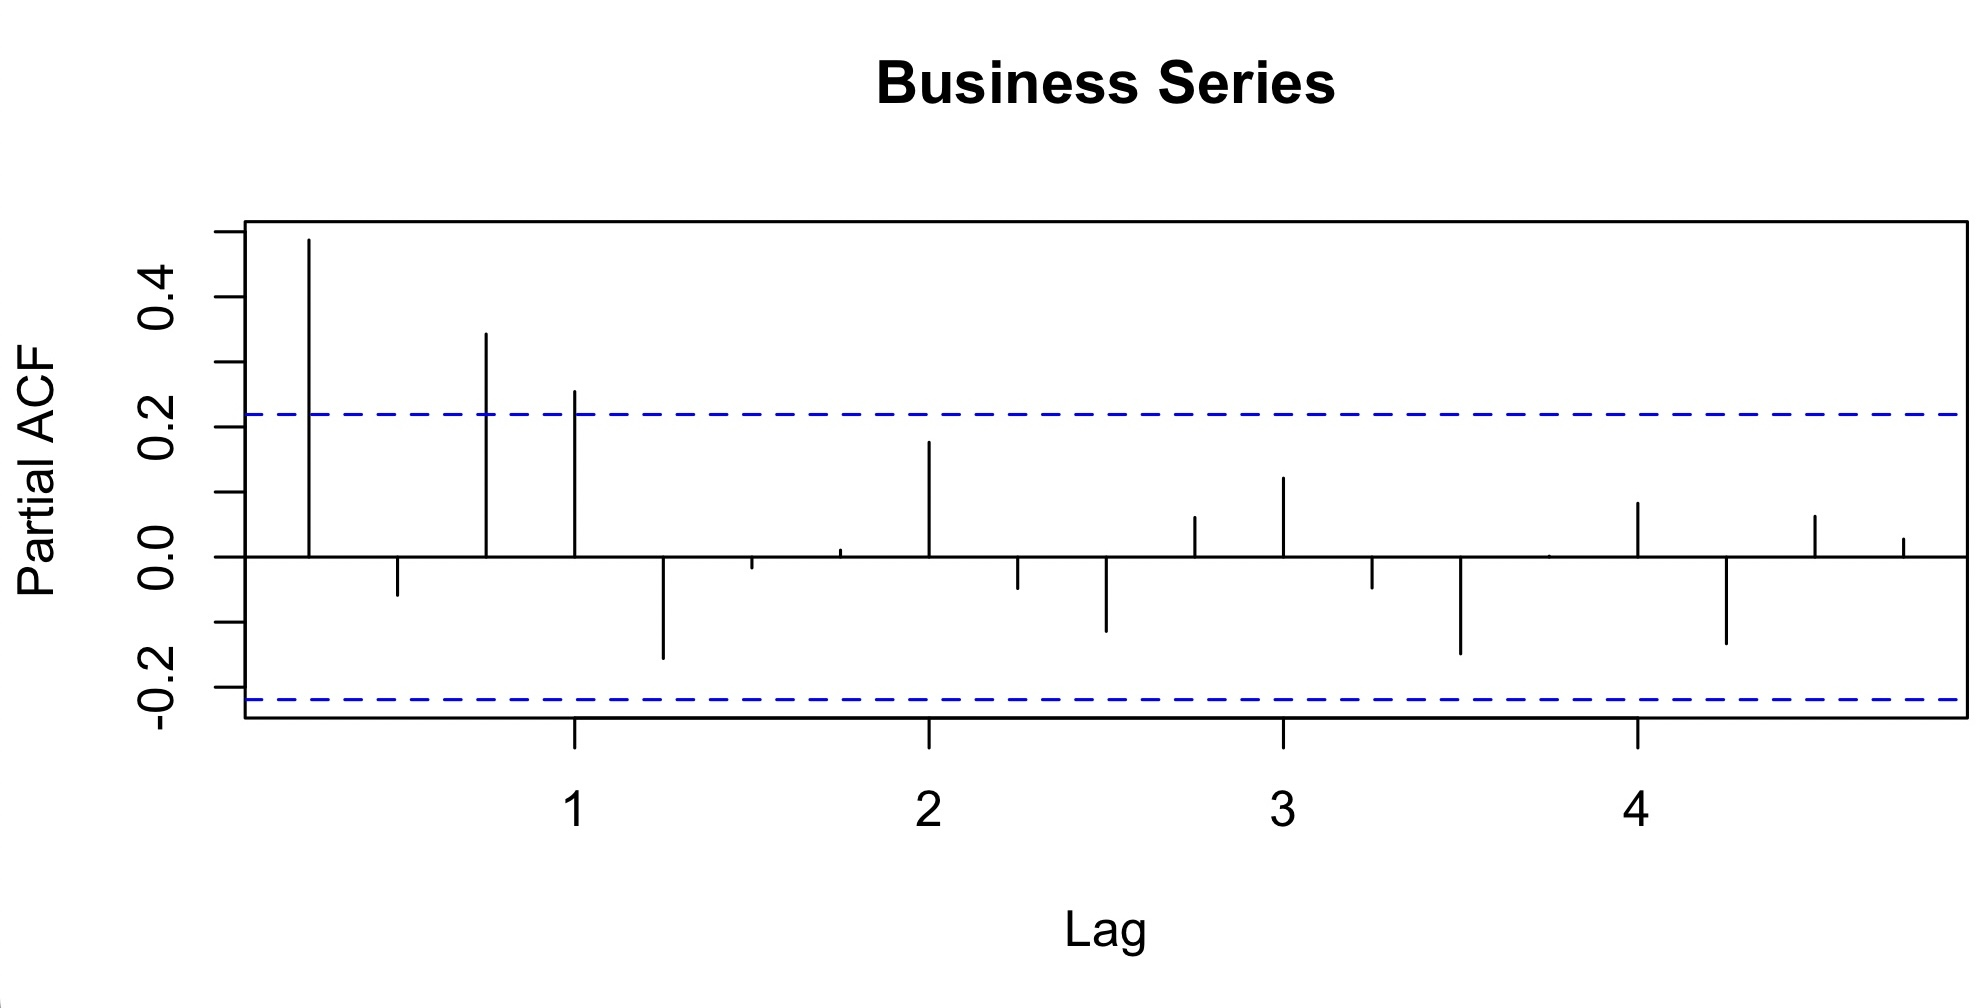
\includegraphics[width=0.65\linewidth]{fig/y1pacf.jpg}
\end{figure}

\noindent The partial autocorrelation at lag 1 is large, similar in size to the lag 1 autocorrelation, as is always the case at lag 1. Beyond lag 1, most of the partial autocorrelations lie within the reference lines, but there are significant spikes too at lag 3 and 4. Persisting correlation at a lag close to the seasonal period, once the effect of shorter lags has been removed, is again typical of a series with a seasonal component still present. \\

\noindent Taken together, the acf and pacf indicate that the business series is \textbf{non-stationary}, and that trend and seasonal effects would need to be identified and removed before the random component could reasonably be treated as stationary.

\subsection{Holiday Series}

\vspace{-0.4cm}
\begin{figure}[H]
    \centering
    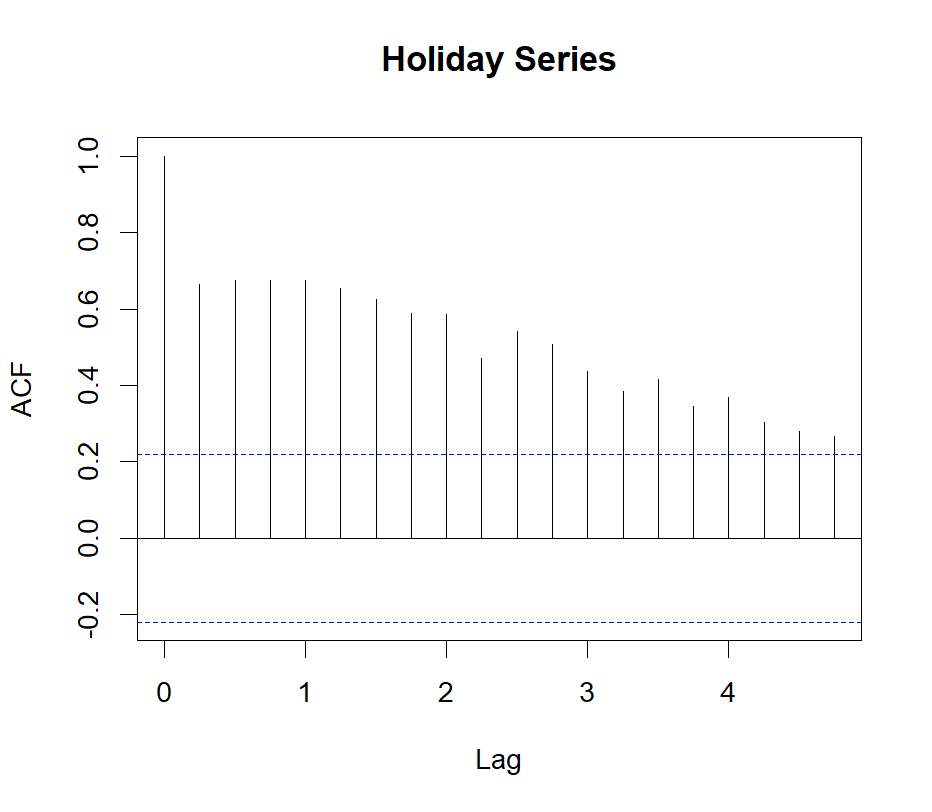
\includegraphics[width=0.65\linewidth]{fig/y2acf.png}
\end{figure}
\vspace{-0.4cm}

\noindent \noindent The ACF does not decay to zero quickly and remains significantly positive over many lags, indicating strong autocorrelation and persistence in the series. The gradual decline of the autocorrelations suggests that the series is unlikely to be stationary. This behaviour is consistent with the upward trend observed in the time plot, where the number of holiday trips increases over time.

\noindent The ACF does not show strong repeating spikes at seasonal lags, suggesting that the seasonal pattern is not dominant in the autocorrelation structure of the original series. Instead, the high autocorrelation across consecutive lags indicates that observations close together in time tend to have similar values. This suggests that the series contains a strong trend component rather than purely random fluctuations.



\vspace{0.4cm}

\begin{figure}[H]
    \centering
    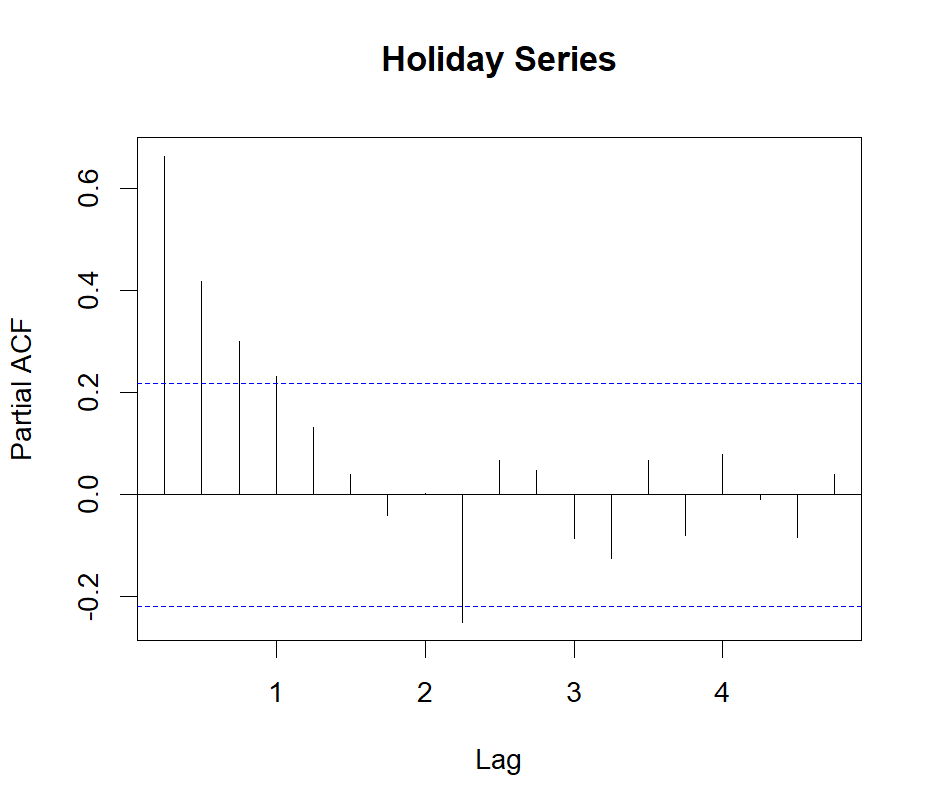
\includegraphics[width=0.65\linewidth]{fig/y2pacf.png}
\end{figure}

\noindent \noindent The PACF shows a large positive spike at lag 1, while most of the remaining partial autocorrelations are within the reference limits, except for a noticeable spike at lag 2. The PACF shows a large spike at lag 1, indicating that the first lag has a strong direct influence on the current observation. Most other lags are insignificant.

\noindent Taken together, the ACF and PACF indicate that the Holiday series is \textbf{non-stationary}, mainly due to the presence of a trend component. Therefore, differencing should be considered to remove the trend and achieve stationarity before fitting an ARIMA or SARIMA model.


% Fit and Compare Models
\section{Fit and Compare Models}
\subsection{Business Series}
Since the Business series is found to be non-stationary,differencing is applied before a model is fitted. A first difference is taken to remove the trend identified previously.
\begin{figure}[H]
    \centering
    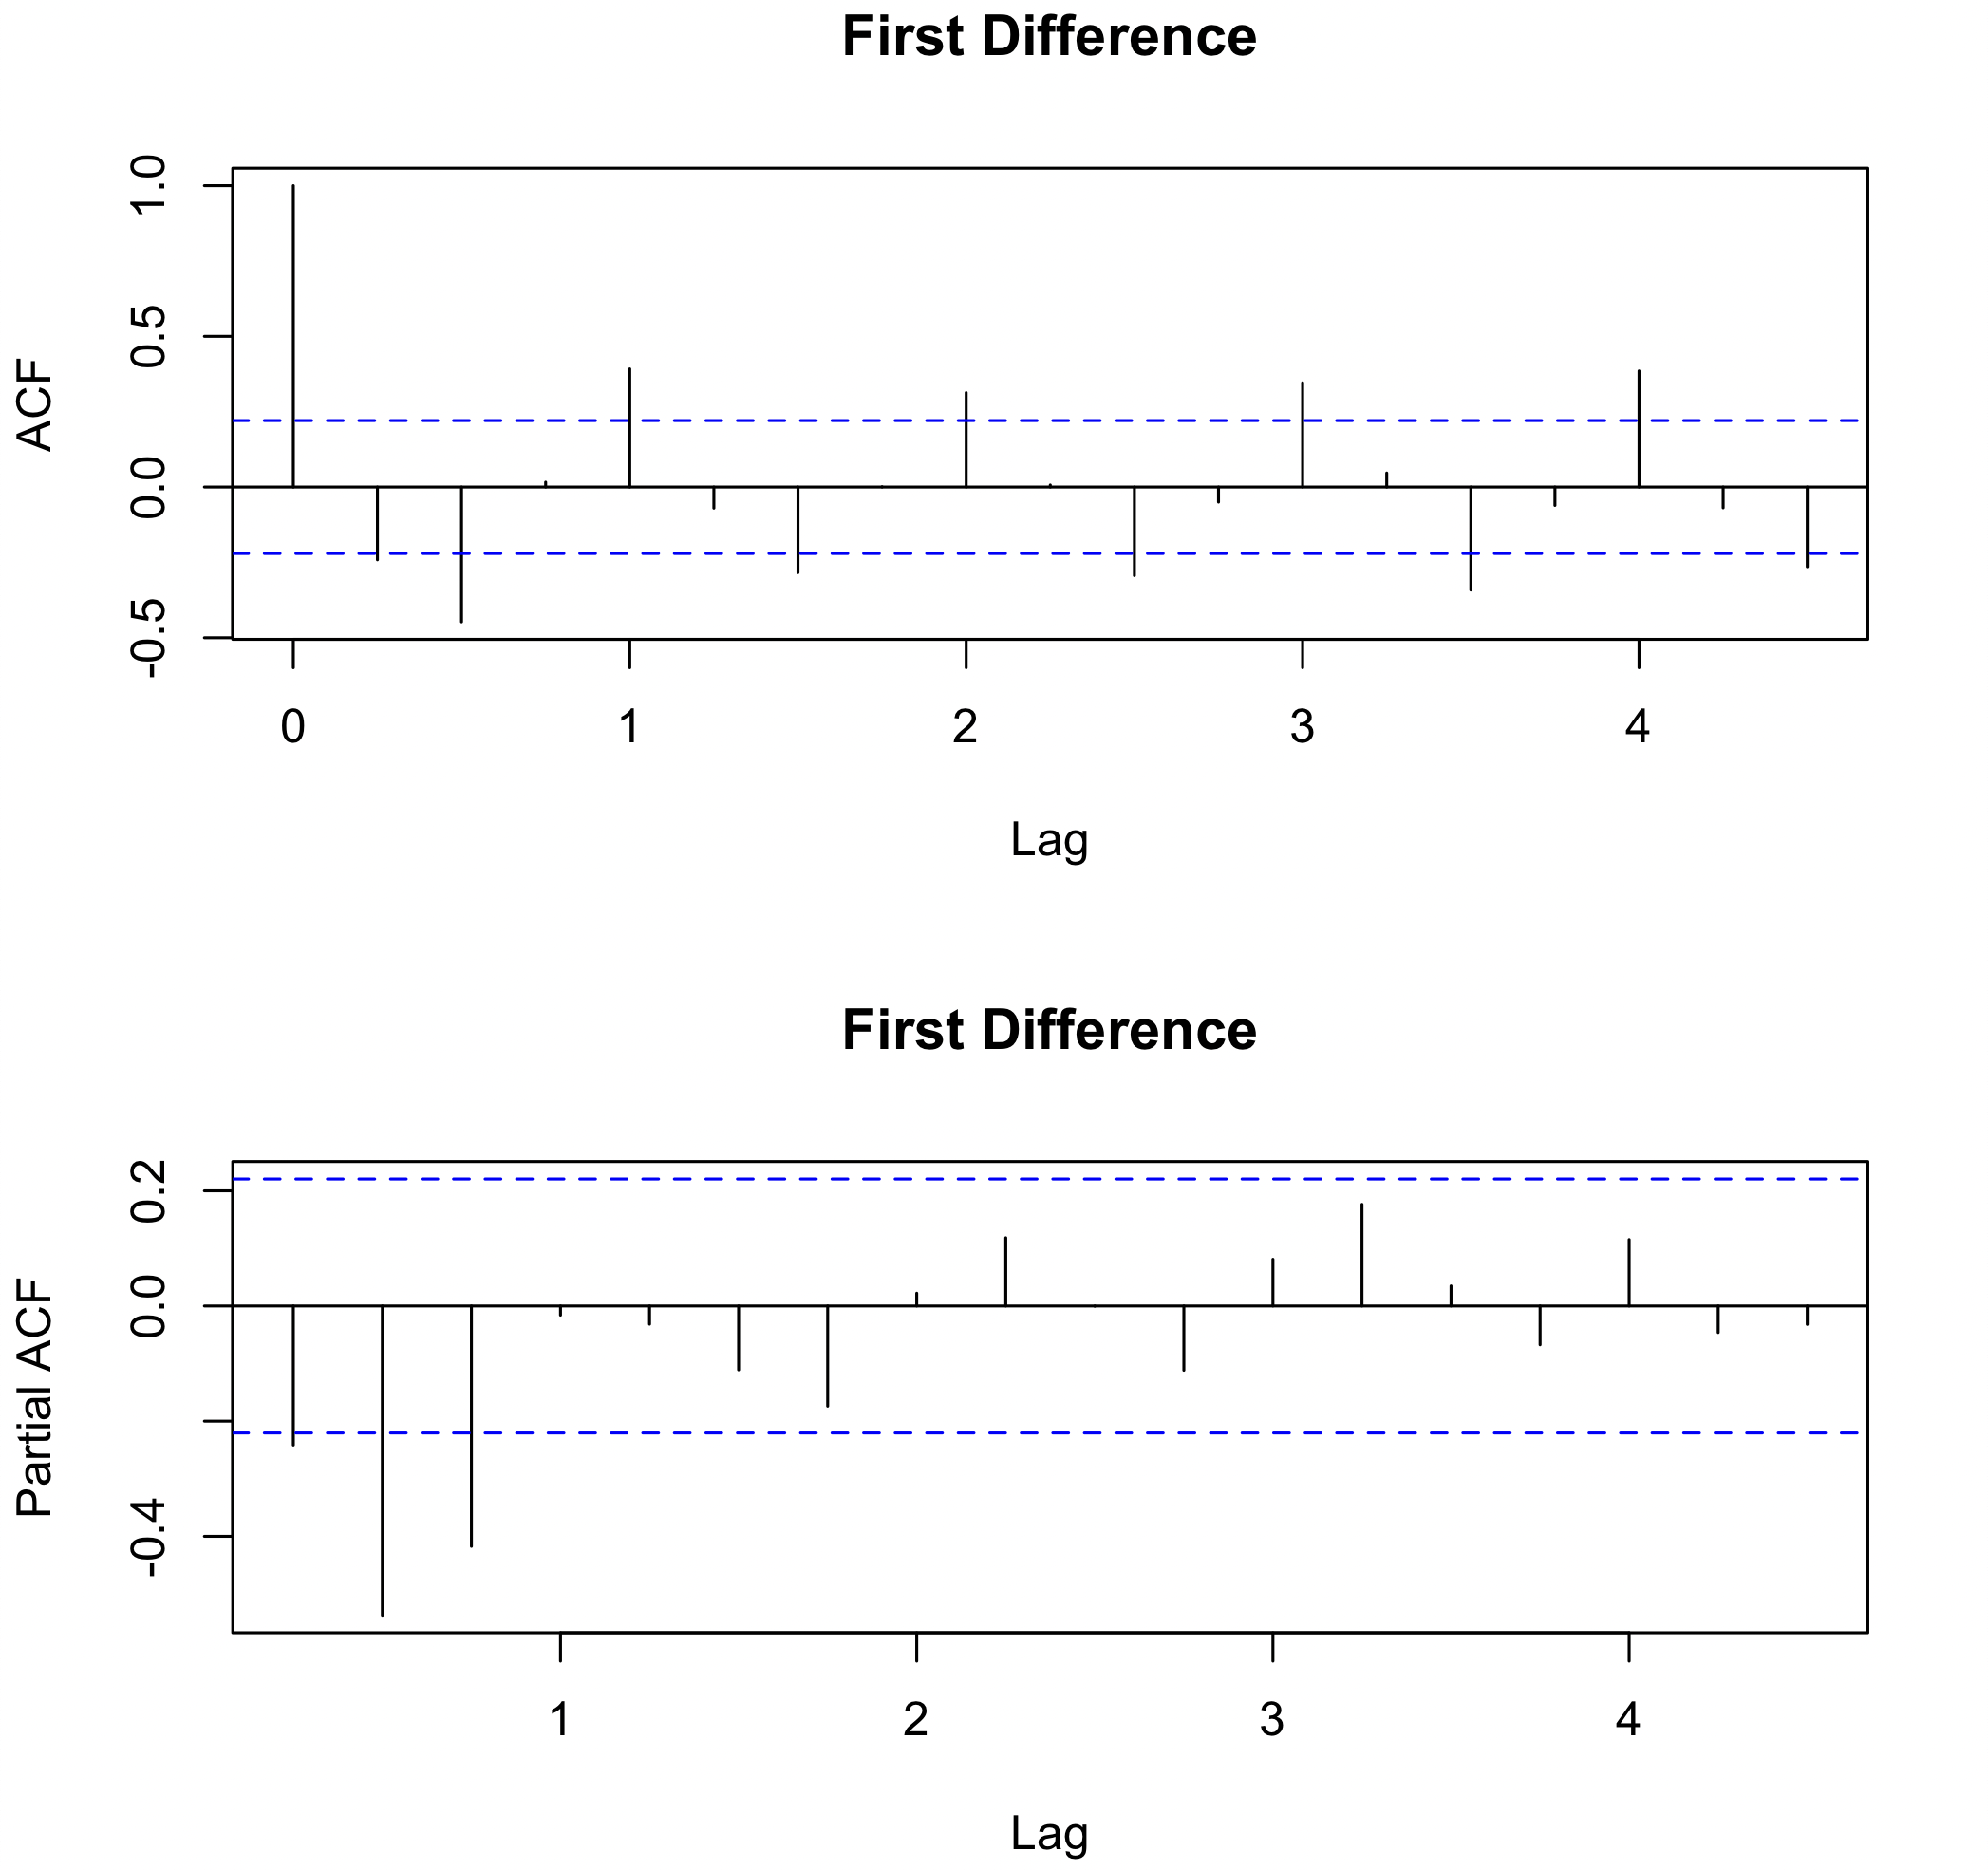
\includegraphics[width=0.5\linewidth]{fig/y1diff.png}
\end{figure}
\vspace{-0.4cm}
\noindent The correlogram of the first difference still shows a repeating pattern of significant autocorrelations, and the seasonal component identified has not been removed.\\
A seasonal difference at lag 4 is therefore applied to the already first-differenced series.
\begin{figure}[H]
    \centering
    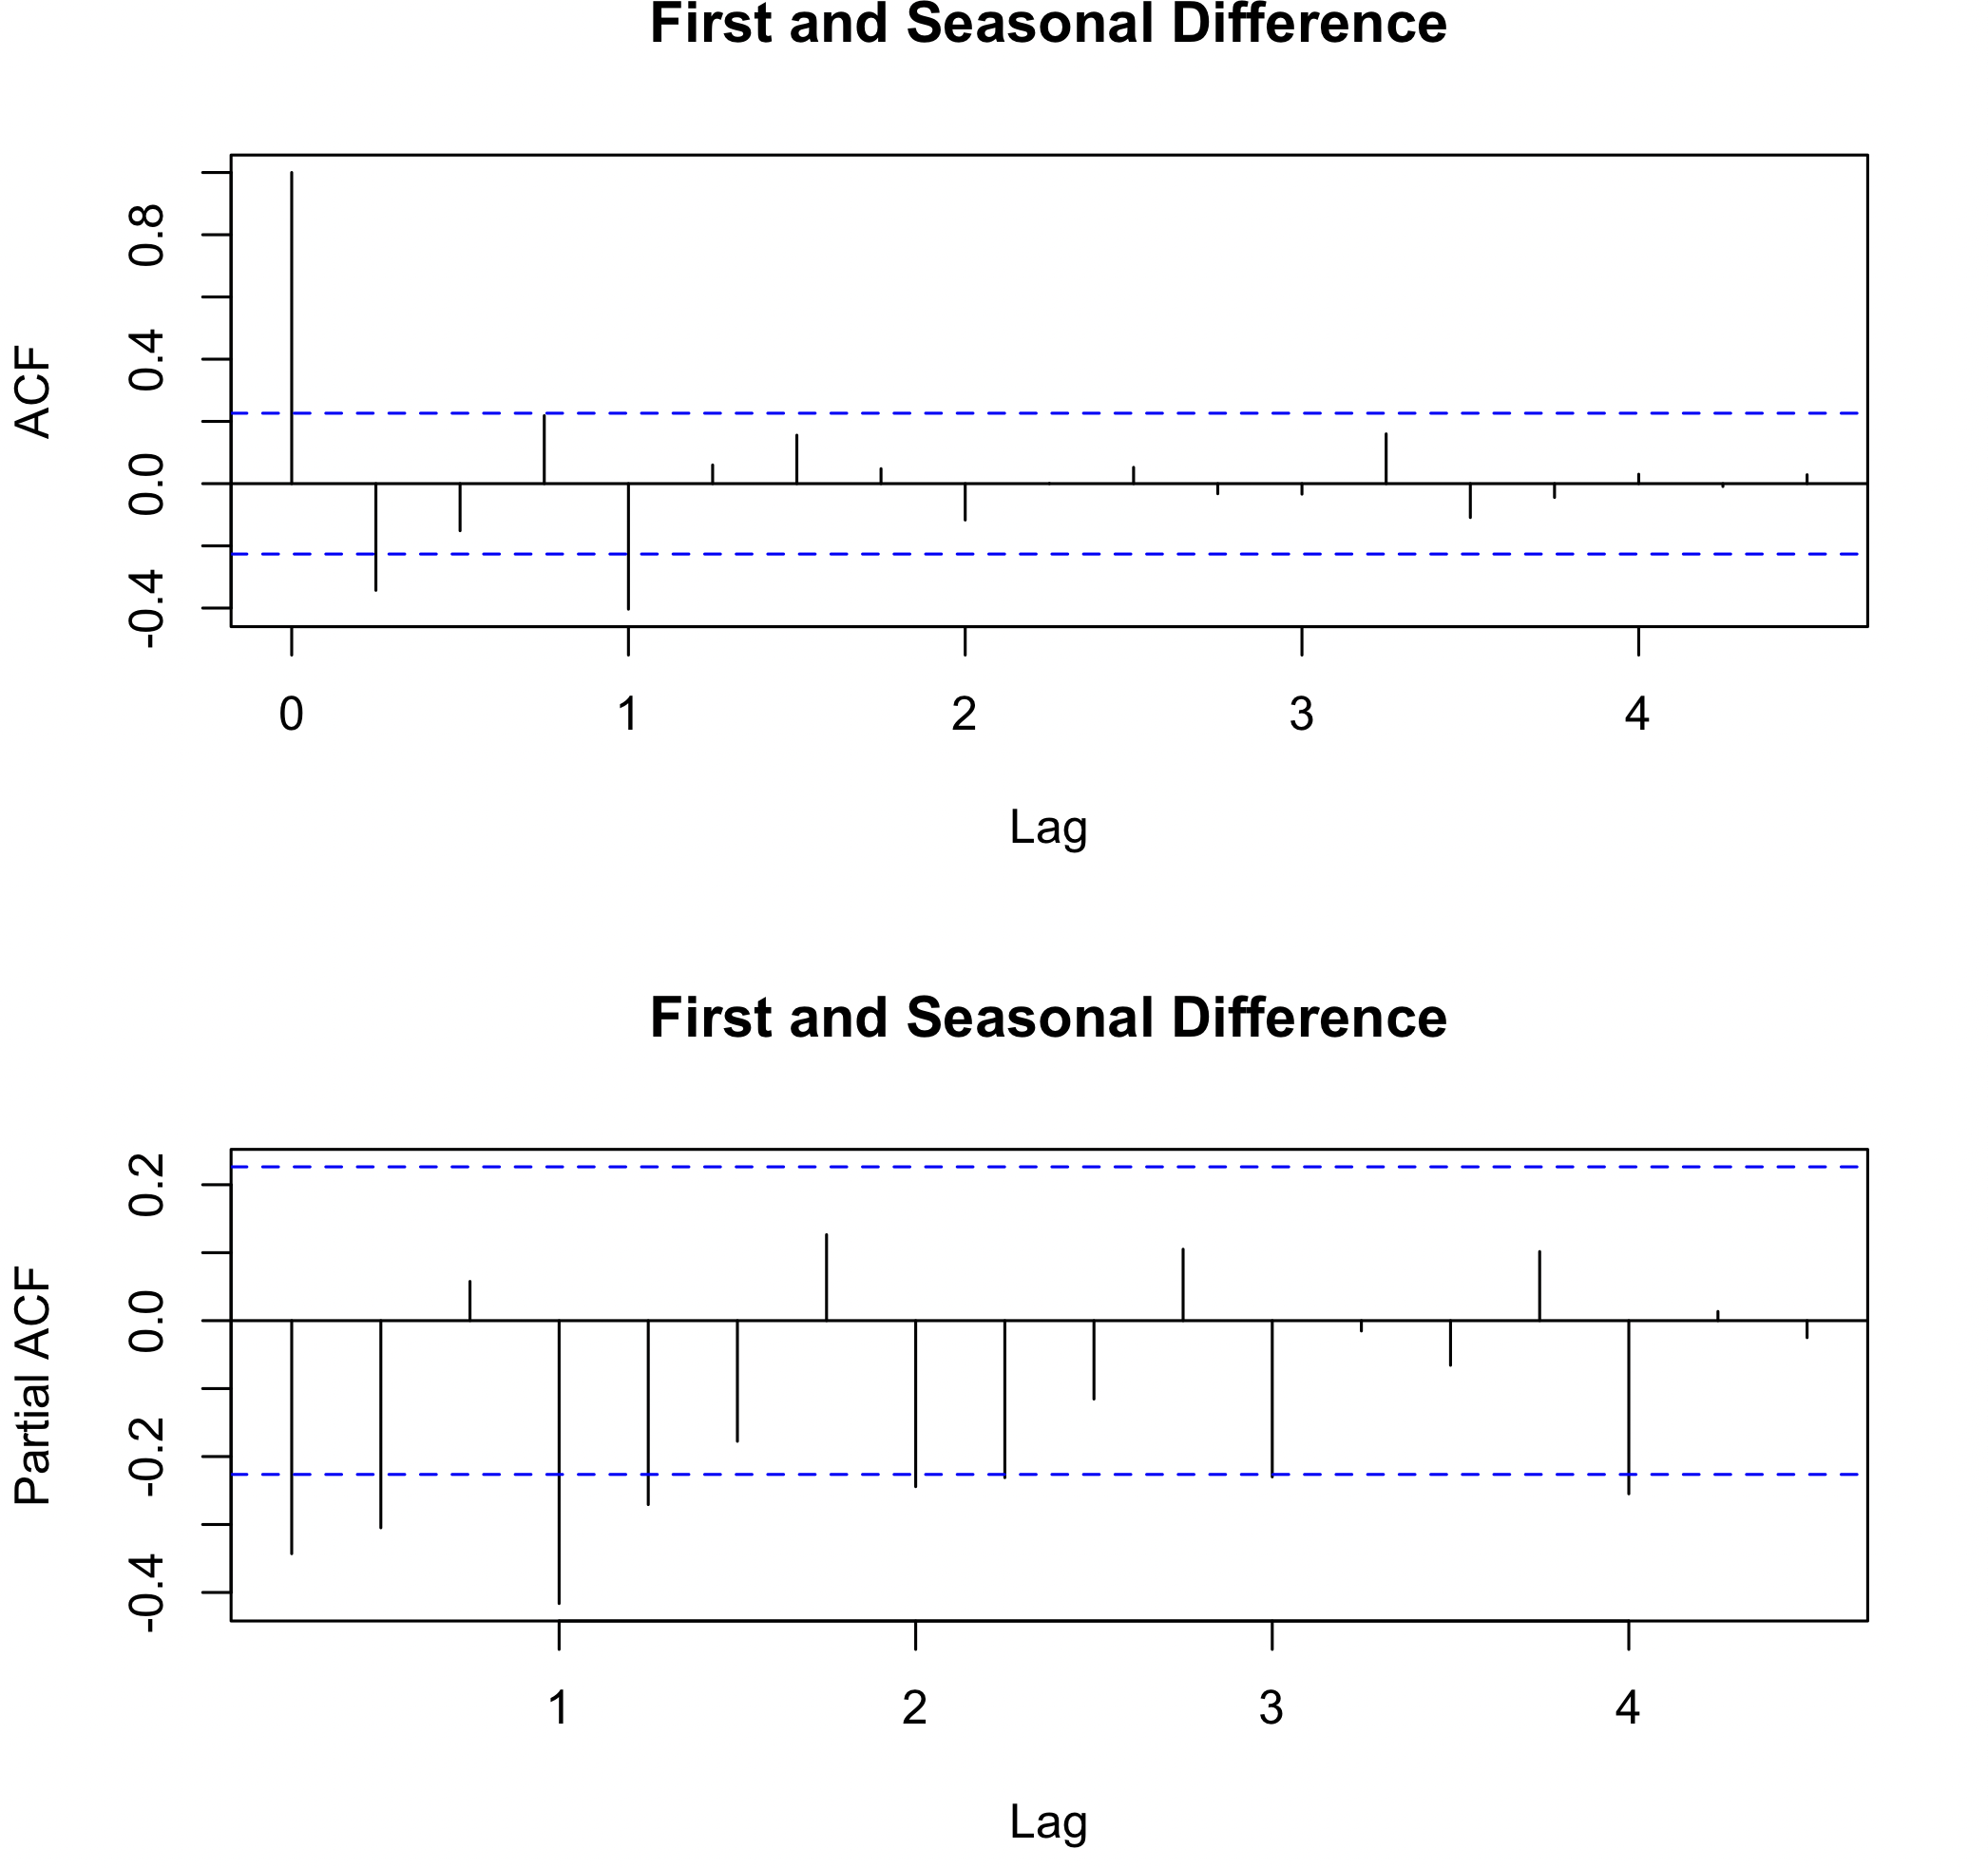
\includegraphics[width=0.5\linewidth]{fig/y1fsdiff.png}
\end{figure}
\noindent The correlogram now decays rapidly, with only a few significant lags and no remaining seasonal pattern, suggesting that d=1 and D=1 are appropriate differencing orders for the ARIMA search.\\
The \texttt{get.best.sarima} function defined in Lecture Notes Ch.7 is then used to identify the optimal SARIMA model.
% \begin{lstlisting}[language=R,basicstyle=\ttfamily\footnotesize]
% get.best.sarima <- function(x.ts, maxord = c(1,1,1,1,1,1))
% {best.aic <- Inf
%   n <- length(x.ts)
%   for(p in 0:maxord[1])for(d in 0:maxord[2]) for(q in 0:maxord[3])
%   for(P in 0:maxord[4])for(D in 0:maxord[5]) for(Q in 0:maxord[6])
%   {fit <- arima(x.ts,order=c(p, d, q),
%                  seasonal=list(order = c(P, D, Q),frequency(x.ts)),
%                  method = "CSS")
%     fit.aic <- -2 * fit$loglik + (log(n) + 1) * length(fit$coef)
%     if (fit.aic < best.aic)
%     {best.aic   <- fit.aic
%       best.fit   <- fit
%       best.order <- c(p, d, q, P, D, Q)}}
%   list(best.aic, best.fit, best.order)}
% \end{lstlisting}
\noindent The function evaluates all model orders up to maxord and selects the one with the lowest CAIC.
% \begin{lstlisting}[language=R]
% y1.best <- get.best.sarima(y1, maxord = c(2,2,2,2,2,2))
% y1.best
% \end{lstlisting}
\vspace{-0.4cm}
\begin{figure}[H]
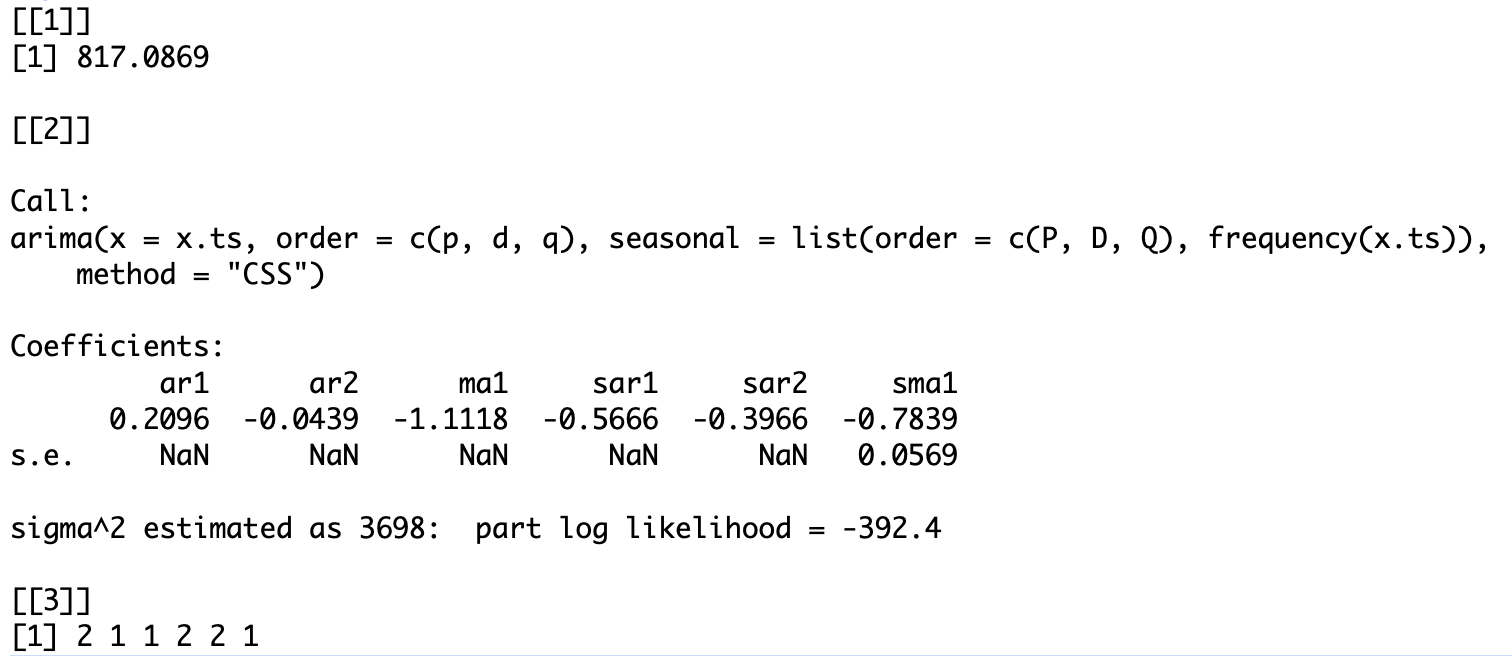
\includegraphics[width=0.75\linewidth]{fig/y1best.png}
\end{figure}
\vspace{-0.4cm}
\noindent Searching up to second order (\texttt{maxord = c(2,2,2,2,2,2)}) selects ARIMA$(2,1,1)(2,2,1)_4$ as the best fit. However, \texttt{confint()} cannot compute $95\%$ confidence intervals for most coefficients due to excessive seasonal differencing ($D=2$) relative to the small sample size ($n=80$). As the parameters are not reliably estimable, the model is not pursued further.
% \begin{lstlisting}[language=R]
% y1.best2 <- get.best.sarima(y1, maxord = c(2,1,2,2,1,2))
% y1.best2
% \end{lstlisting}
\vspace{-0.4cm}
\begin{figure}[H]
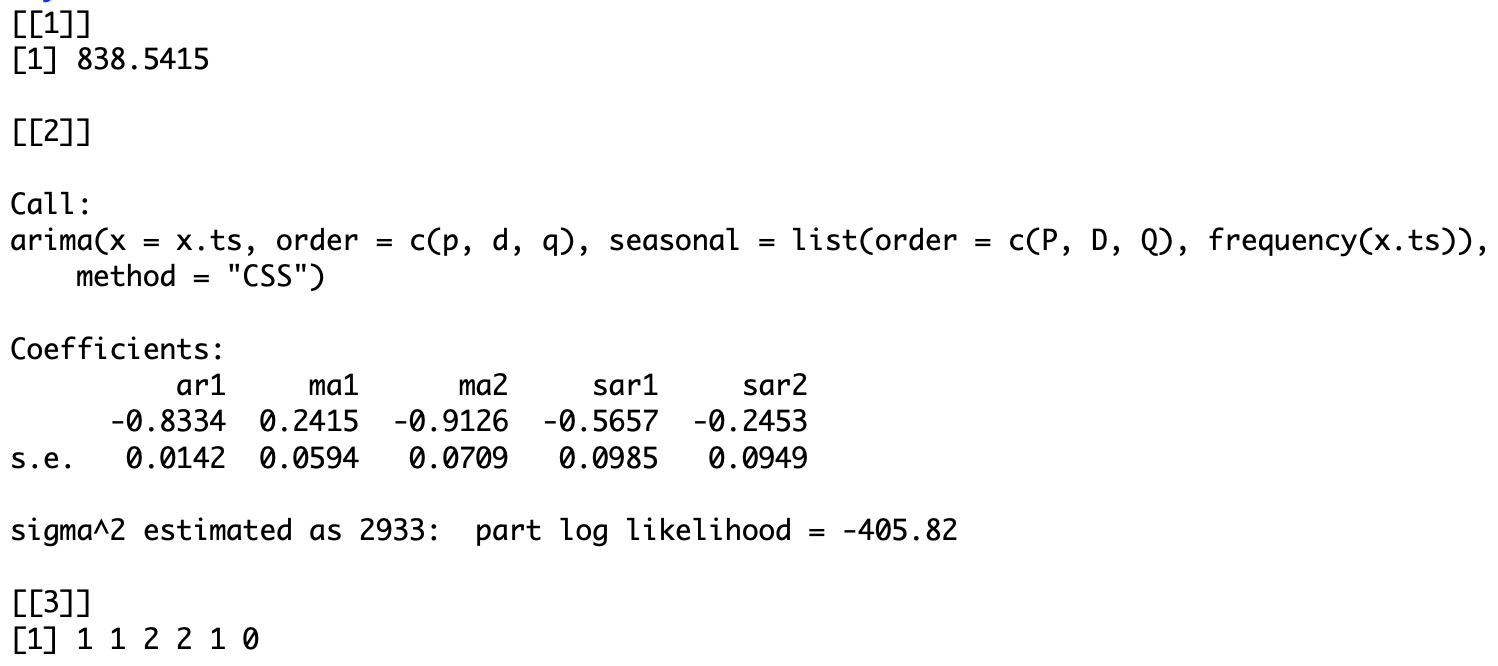
\includegraphics[width=0.75\linewidth]{fig/y1best2.png}
\end{figure}
\vspace{-0.4cm}
\noindent Restricting the search to at most one difference at each level ($d \leq 1$, $D \leq 1$), consistent with the differencing established above, identifies ARIMA$(1, 1, 2)(2, 1, 0)_4$ as the best-fitting model.
% \begin{lstlisting}[language=R]
% y1.sarima <- arima(y1, order = c(1,1,2),
%                 seasonal = list(order = c(2,1,0), 4),
%                 method = "CSS")
% y1.sarima
% \end{lstlisting}
\begin{figure}[H]
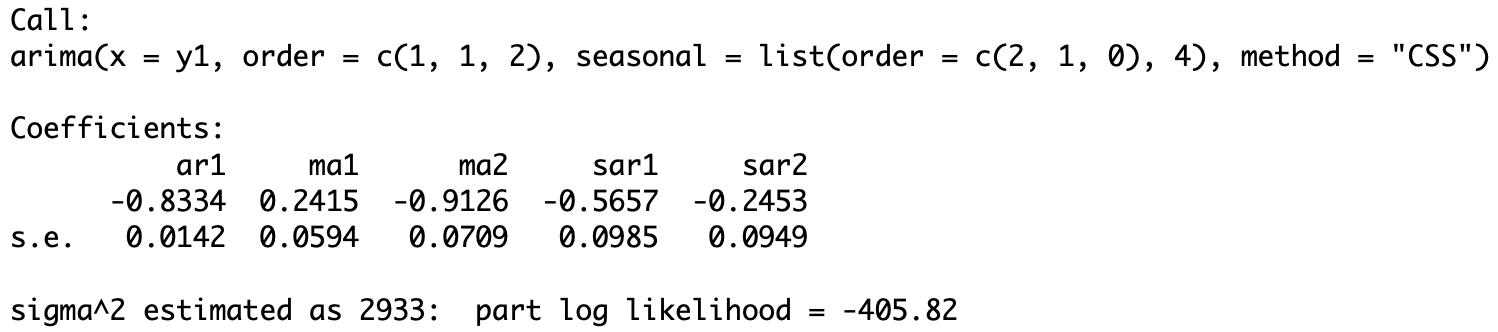
\includegraphics[width=0.75\linewidth]{fig/y1coef.png}
\end{figure}
\vspace{-0.4cm}
% \begin{lstlisting}
% confint(y1.safrima)
% \end{lstlisting}
\vspace{-0.4cm}
\begin{figure}[H]
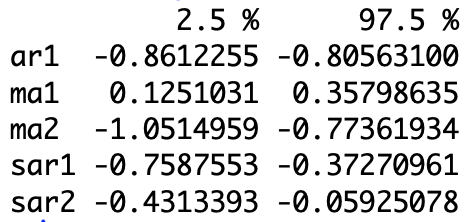
\includegraphics[width=0.25\linewidth]{fig/y1ci.png}
\end{figure}
\noindent All five coefficients are significantly different from zero, as none of the confidence intervals include zero; hence, no terms are removed. The fitted model with $\sigma^2 = 2933$ is
\vspace{-0.5cm}
\begin{align*}
x_t - x_{t-1} &= -0.8334(x_{t-1} - x_{t-2}) - 0.5657(x_{t-4} - x_{t-5}) - 0.2453(x_{t-8} - x_{t-9}) \\
&\quad + w_t + 0.2415w_{t-1} - 0.9126w_{t-2}.
\end{align*}
% \begin{lstlisting}[language=R]
% acf(resid(y1.sarima)^2, main="Squared Residuals")
% \end{lstlisting}
\vspace{-0.5cm}
\begin{figure}[H]
    \centering
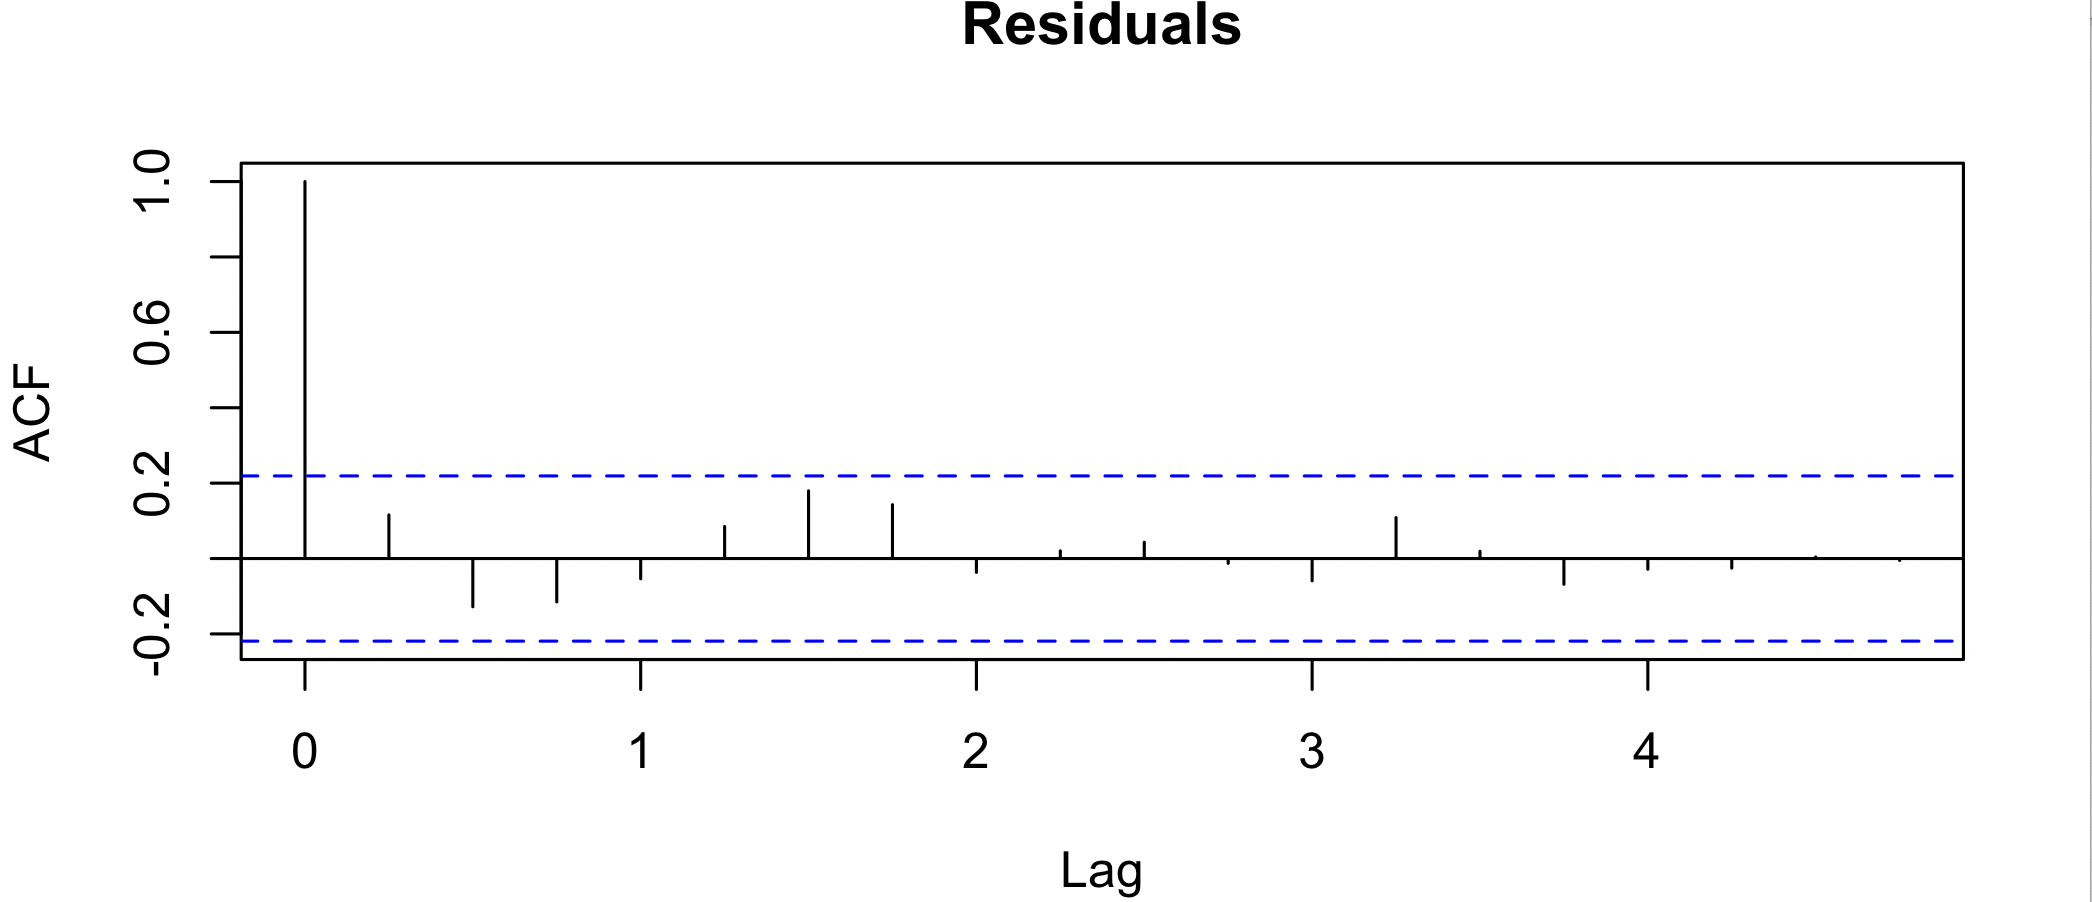
\includegraphics[width=0.75\linewidth]{fig/y1qr.png}
\end{figure}

\noindent The residual correlogram shows no significant autocorrelation, indicating white-noise behaviour and adequate model fit across trend and seasonality.
The \textbf{ARIMA$(1, 1, 2)(2, 1, 0)_4$} model is therefore selected as the final specification for the Business series.


\subsection{Holiday Series}

Since the Holiday series is found to be non-stationary, a first difference is applied before fitting the model to remove the trend identified previously.

\begin{figure}[H]
    \centering
    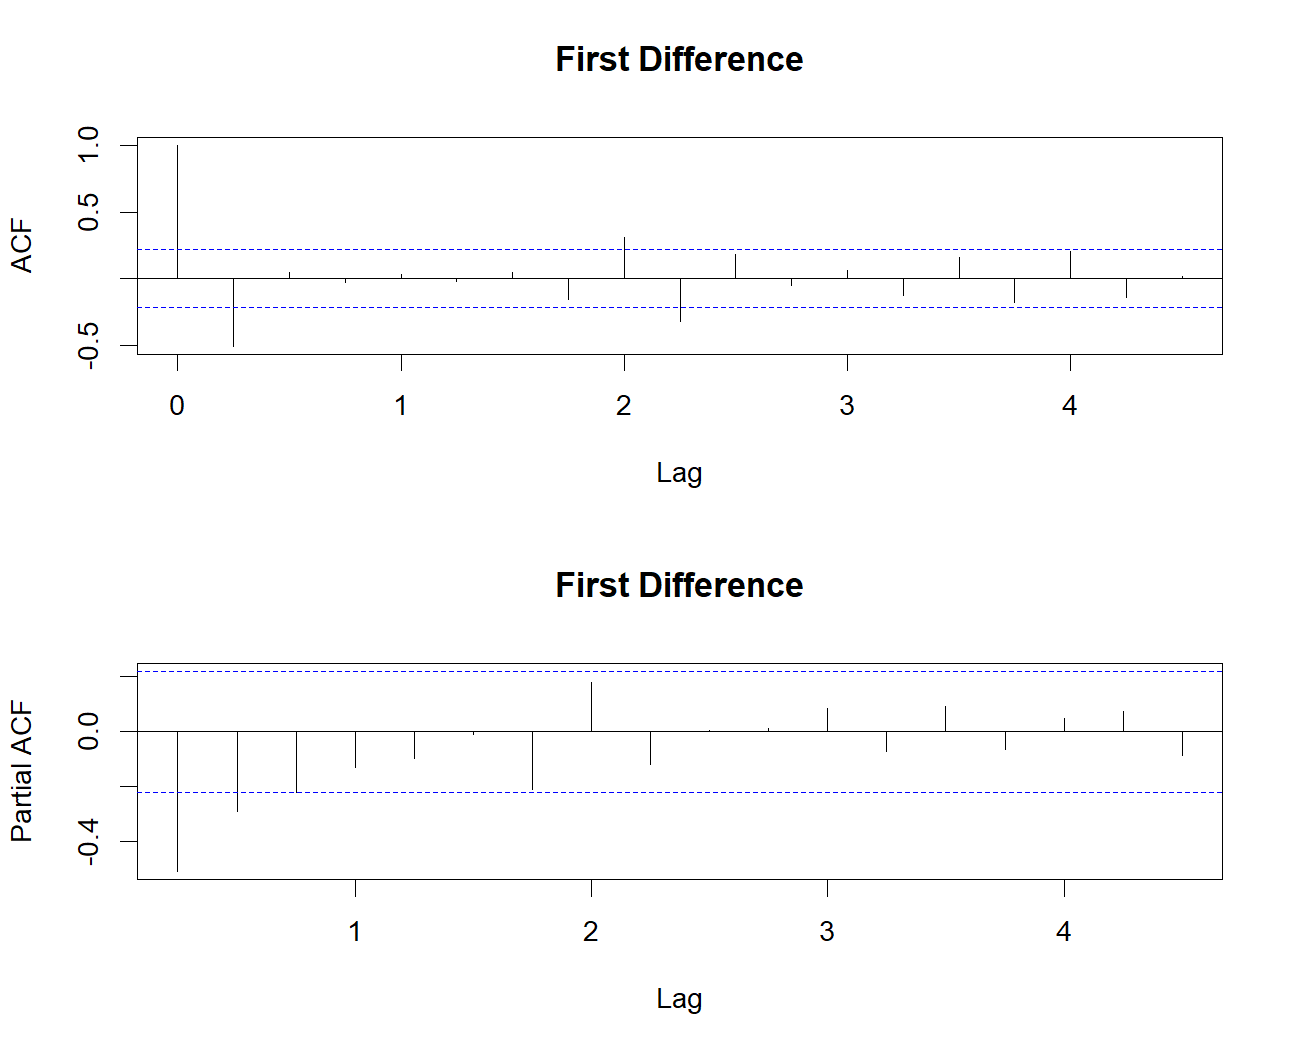
\includegraphics[width=0.75\linewidth]{fig/y2diff.png}
\end{figure}

\noindent The correlogram of the first-differenced series shows that the autocorrelations are substantially reduced, indicating that the trend has been largely removed. However, several significant autocorrelations remain at seasonal lags, suggesting that the seasonal component has not been completely removed. A seasonal difference at lag 4 is therefore applied to the first-differenced series.

\begin{figure}[H]
    \centering
    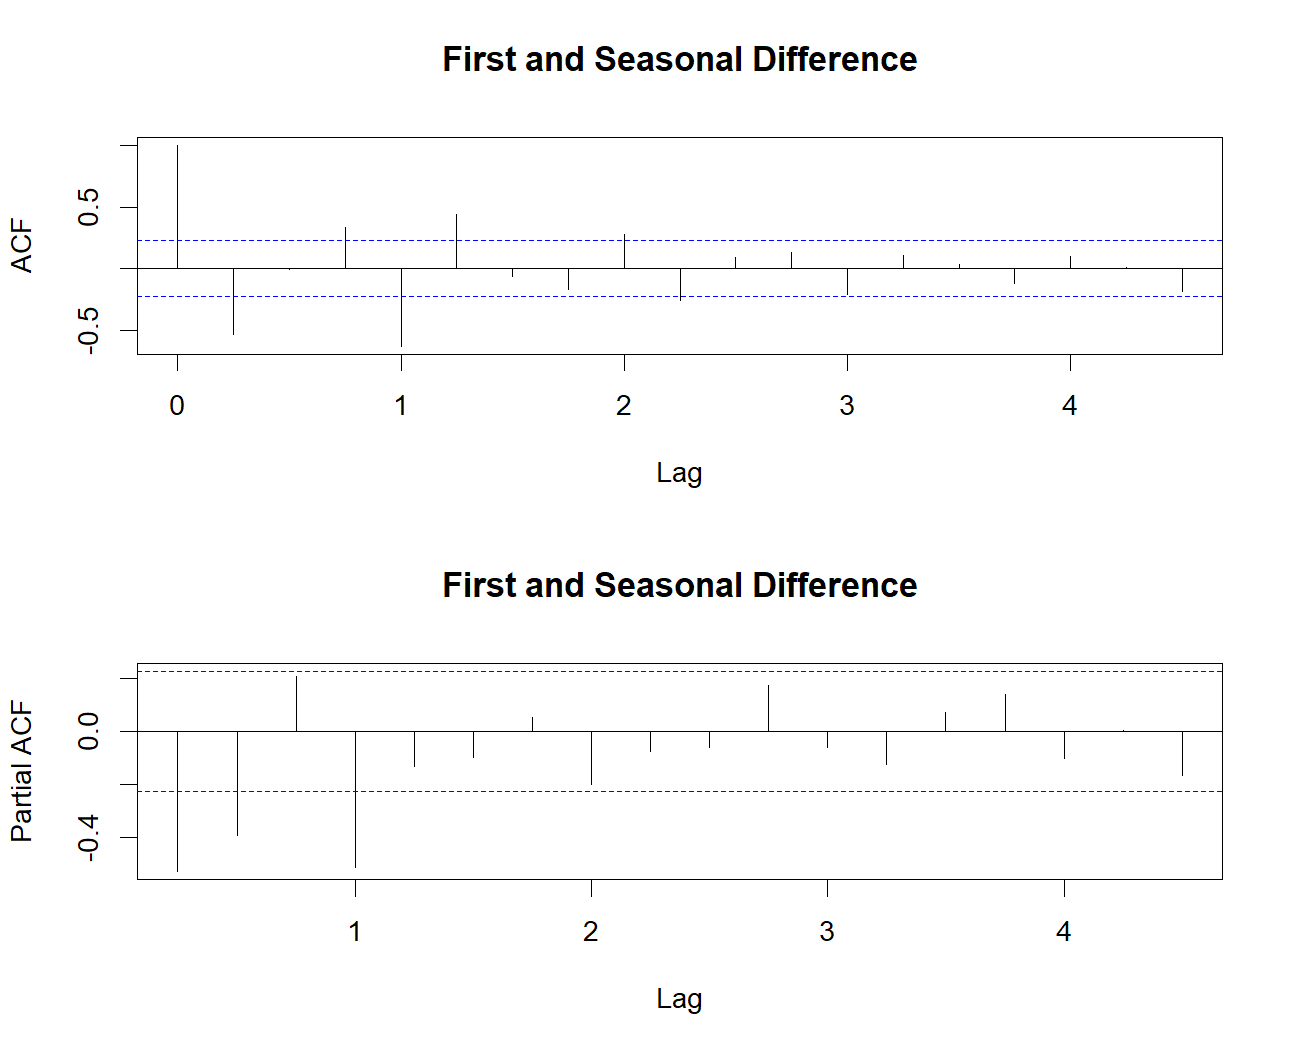
\includegraphics[width=0.75\linewidth]{fig/y2fsdiff.png}
\end{figure}

\noindent After applying both first and seasonal differencing, the autocorrelations decay more rapidly and the seasonal pattern is substantially reduced. Although some significant spikes remain, the differenced series is closer to stationarity. Therefore, \(d=1\) and \(D=1\) are considered appropriate starting values for the SARIMA model search.

\noindent The \texttt{get.best.sarima} function defined in Lecture Notes Ch.7 is then used to identify the optimal SARIMA model.


\begin{figure}[H]
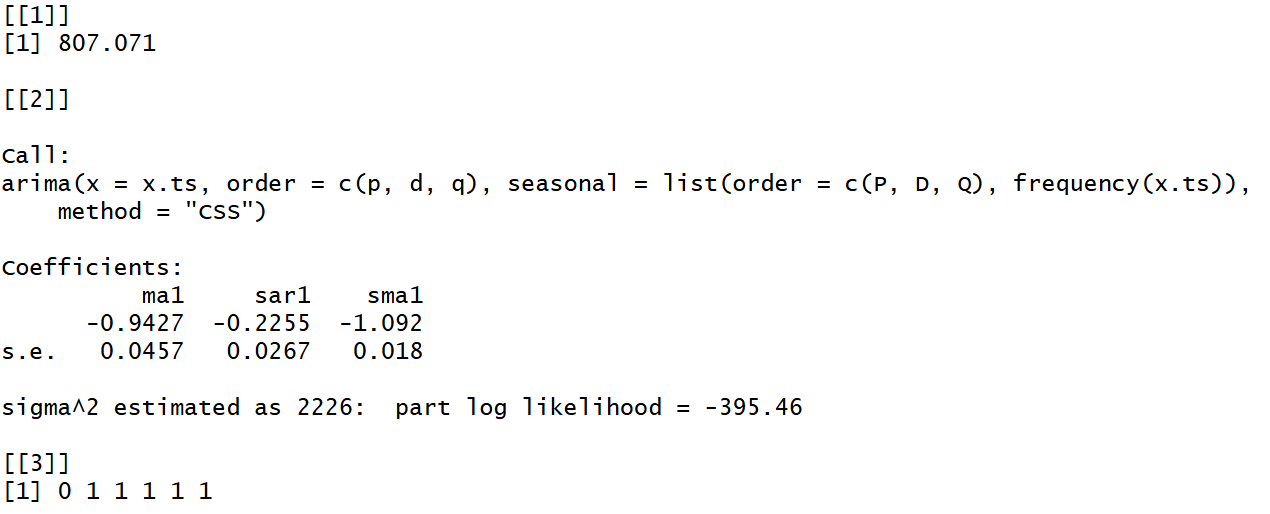
\includegraphics[width=0.75\linewidth]{fig/y2coef.png}
\end{figure}
\vspace{-0.4cm}

\begin{figure}[H]
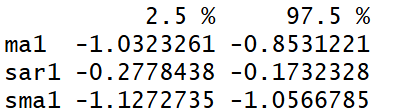
\includegraphics[width=0.25\linewidth]{fig/y2ci.png}
\end{figure}

\noindent All three coefficients are significantly different from zero, as none of the confidence intervals include zero; hence, no terms are removed. The fitted model with $\sigma^2 = 2226$ is

\vspace{-0.5cm}

\begin{align*}
x_t-x_{t-1}-x_{t-4}+x_{t-5}
&= w_t -0.9427w_{t-1}\\
&\quad -0.2255(x_{t-4}-x_{t-5})
-1.092w_{t-4}.
\end{align*}

\vspace{-0.5cm}

\begin{figure}[H]
    \centering
    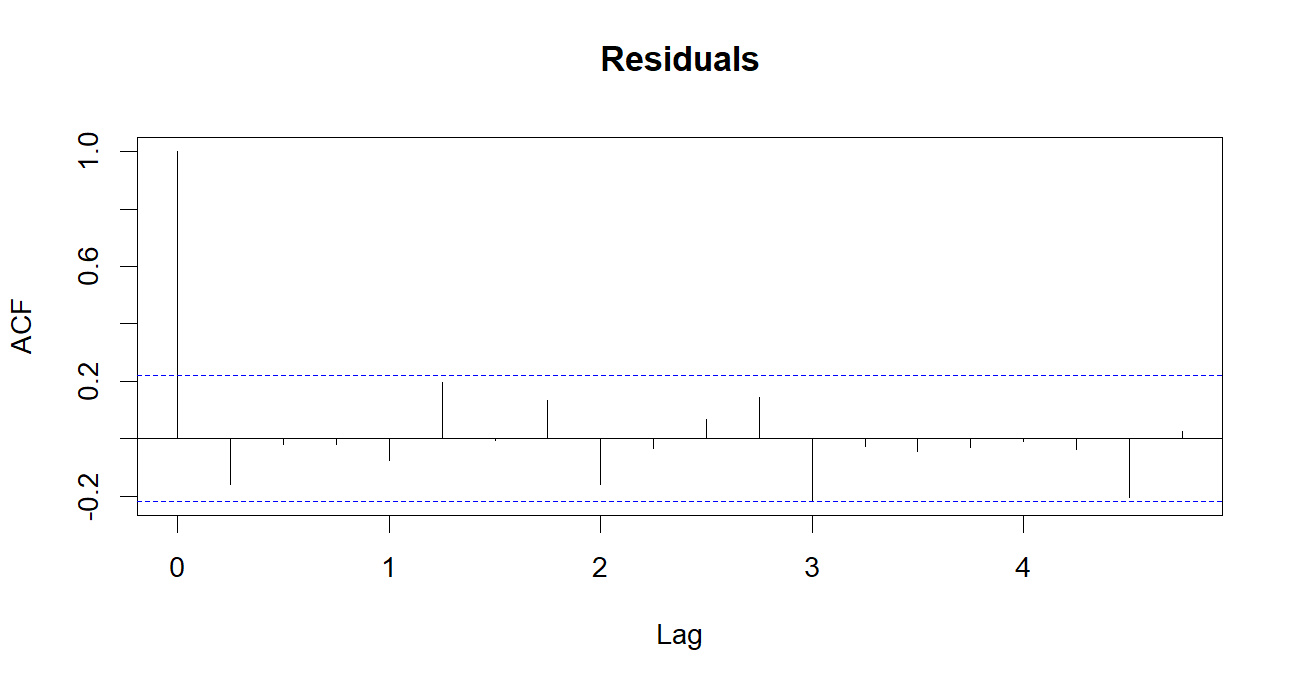
\includegraphics[width=0.75\linewidth]{fig/y2qr.png}
\end{figure}

\noindent The residual correlogram shows no significant autocorrelation, indicating white-noise behaviour and suggesting that the model adequately captures the trend and seasonal patterns in the Holiday series. The \textbf{ARIMA$(0,1,1)(1,1,1)_4$} model is therefore selected as the final specification for the Holiday series.




\subsection{Conclusion of the Two Series}

\noindent In conclusion, both Business and Holiday series were found to be non-stationary and required first and seasonal differencing before model fitting. The final selected models are ARIMA$(1,1,2)(2,1,0)_4$ for the Business series and ARIMA$(0,1,1)(1,1,1)_4$ for the Holiday series. Both models have significant coefficients and their residuals show white-noise behaviour, indicating that the models provide adequate fits for forecasting future quarterly trips.
% Forecasting
\section{Forecasting}
\subsection{Business Series}
Adopting ARIMA$(1, 1, 2)(2, 1, 0)_4$ as the fitted model for the Business series, forecasts of the number of business trips for the next 8 quarters (2018 Q1 to 2019 Q4) are obtained using the $\texttt{predict}$ function.
\vspace{-0.4cm}
\begin{figure}[H]
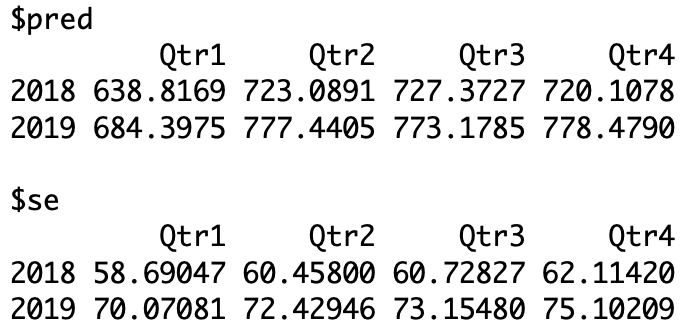
\includegraphics[width=0.4\linewidth]{fig/y1pred.png}
\end{figure}

\vspace{-0.4cm}
\begin{figure}[H]
    \centering
    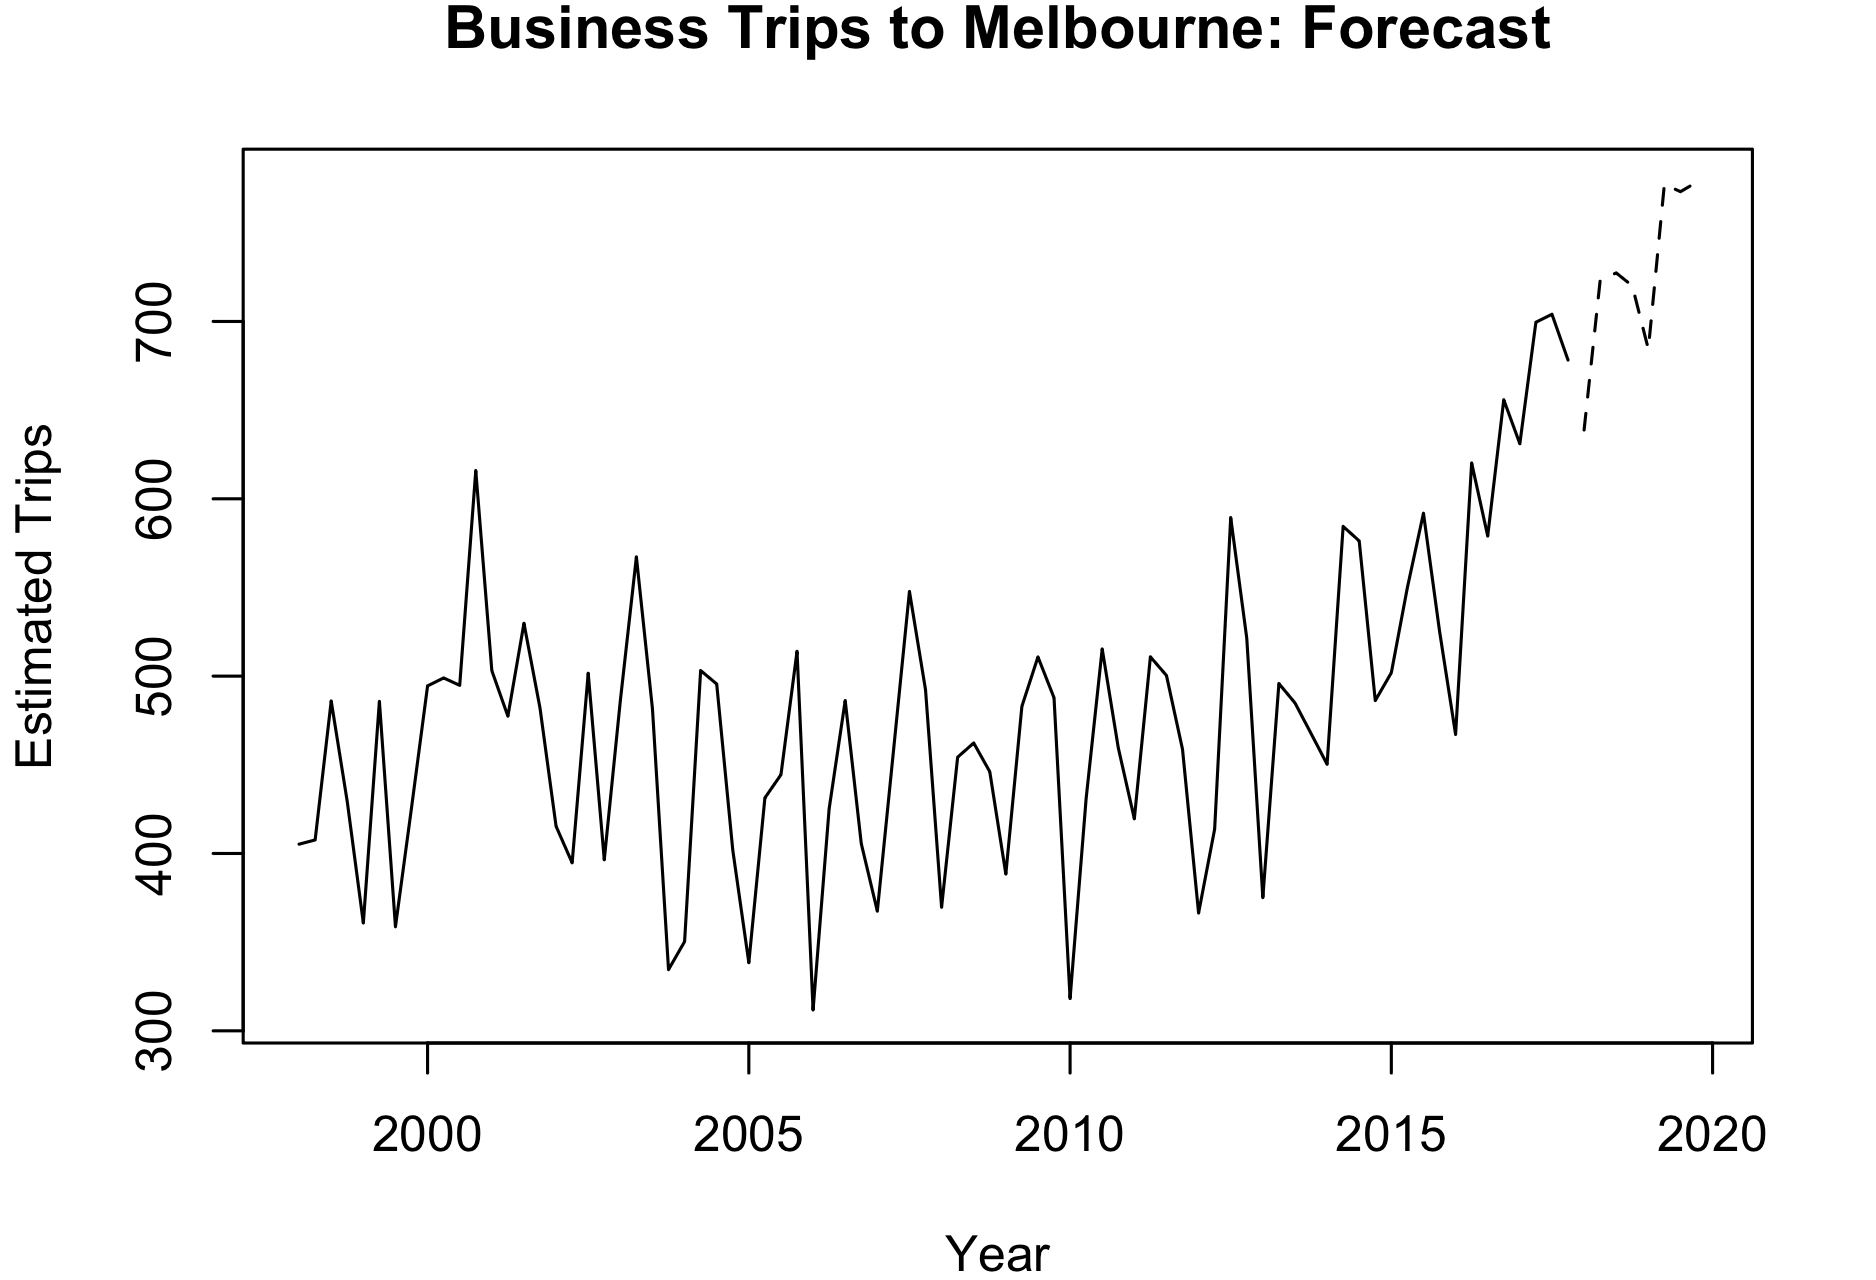
\includegraphics[width=0.65\linewidth]{fig/y1frc.png}
\end{figure}

\noindent The forecasts continue the upward trend and quarterly seasonal pattern established over the observation period, with trips lowest in Q1 of each forecast year and highest around Q2–Q3, consistent with the seasonal pattern identified previously.

\begin{table}[H]
\centering
\begin{tabular}{lccc}
\hline
Time & Forecast & Lower 95\% & Upper 95\% \\
\hline
2018 Q1 & 638.8 & 523.8 & 753.8 \\
2018 Q2 & 723.1 & 604.6 & 841.6 \\
2018 Q3 & 727.4 & 608.3 & 846.4 \\
2018 Q4 & 720.1 & 598.4 & 841.9 \\
2019 Q1 & 684.4 & 547.1 & 821.7 \\
2019 Q2 & 777.4 & 635.5 & 919.4 \\
2019 Q3 & 773.2 & 629.8 & 916.6 \\
2019 Q4 & 778.5 & 631.3 & 925.7 \\
\hline
\end{tabular}
\end{table}

\noindent The prediction intervals increased steadily, from approximately 230 trips at one-quarter ahead to about 294 trips at eight-quarters ahead, reflecting the greater uncertainty attached to forecasts made further into the future.

\noindent These forecasts assume that the trend and seasonal pattern observed up to 2017 Q4 continue unchanged. Any structural changes in the tourism market, such as shifts in business travel behaviour, may cause actual values to deviate from these forecasts.


\subsection{Holiday Series}

Adopting the fitted seasonal ARIMA model for the Holiday series, forecasts of the number of holiday trips for the next 8 quarters (2018 Q1 to 2019 Q4) are obtained using the $\texttt{predict}$ function.

\vspace{-0.4cm}
\begin{figure}[H]
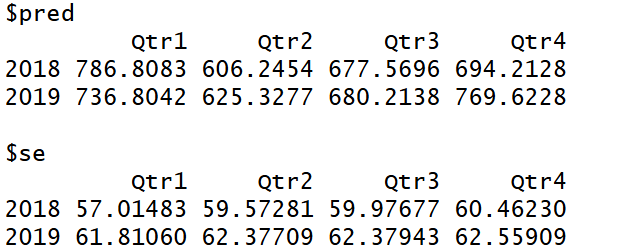
\includegraphics[width=0.4\linewidth]{fig/y2pred.png}
\end{figure}

\vspace{-0.4cm}
\begin{figure}[H]
    \centering
    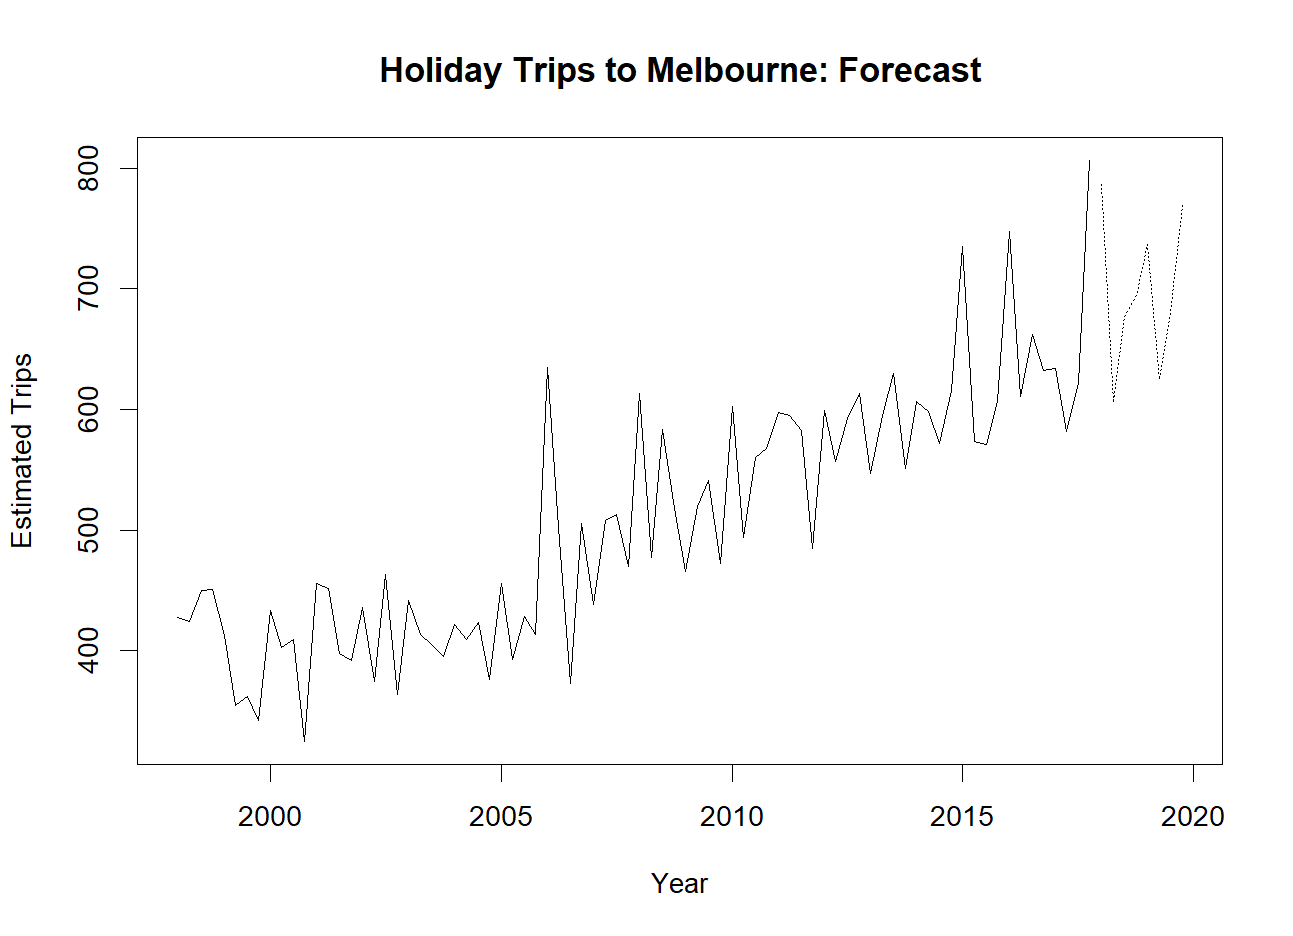
\includegraphics[width=0.7\linewidth]{fig/y2frc.png}
\end{figure}

\noindent The forecasts preserve the seasonal pattern observed in the Holiday series. The predicted values show a recurring quarterly pattern, with higher numbers of holiday trips occurring around Q1 and Q4, while relatively lower values are observed in Q2. This behaviour is consistent with the seasonal variation identified from the previous time series analysis.

\begin{table}[H]
\centering
\begin{tabular}{lccc}
\hline
Time & Forecast & Lower 95\% & Upper 95\% \\
\hline
2018 Q1 & 786.8 & 675.1 & 898.5 \\
2018 Q2 & 606.2 & 489.5 & 723.0 \\
2018 Q3 & 677.6 & 559.9 & 795.2 \\
2018 Q4 & 694.2 & 575.7 & 812.7 \\
2019 Q1 & 736.8 & 615.6 & 858.0 \\
2019 Q2 & 625.3 & 503.1 & 747.6 \\
2019 Q3 & 680.2 & 557.9 & 802.5 \\
2019 Q4 & 769.6 & 646.9 & 892.3 \\
\hline
\end{tabular}
\end{table}

\noindent The prediction intervals become wider as the forecast horizon increases. The interval width increases from approximately 223 trips for the first forecast quarter to around 245 trips for the final forecast quarter, indicating increasing uncertainty for forecasts further into the future.

\noindent These forecasts assume that the historical seasonal pattern of holiday travel continues unchanged. However, future holiday travel demand may be influenced by external factors such as economic conditions, tourism trends, and unexpected events, which may cause actual values to deviate from the forecasts.

% Volatility Check
\pagebreak
\section{Volatility}
\subsection{Business Series}
% \begin{lstlisting}[language=R]
% acf(resid(y1.sarima)^2, main="Squared Residuals")
% \end{lstlisting}
\begin{figure}[H]
    \centering
    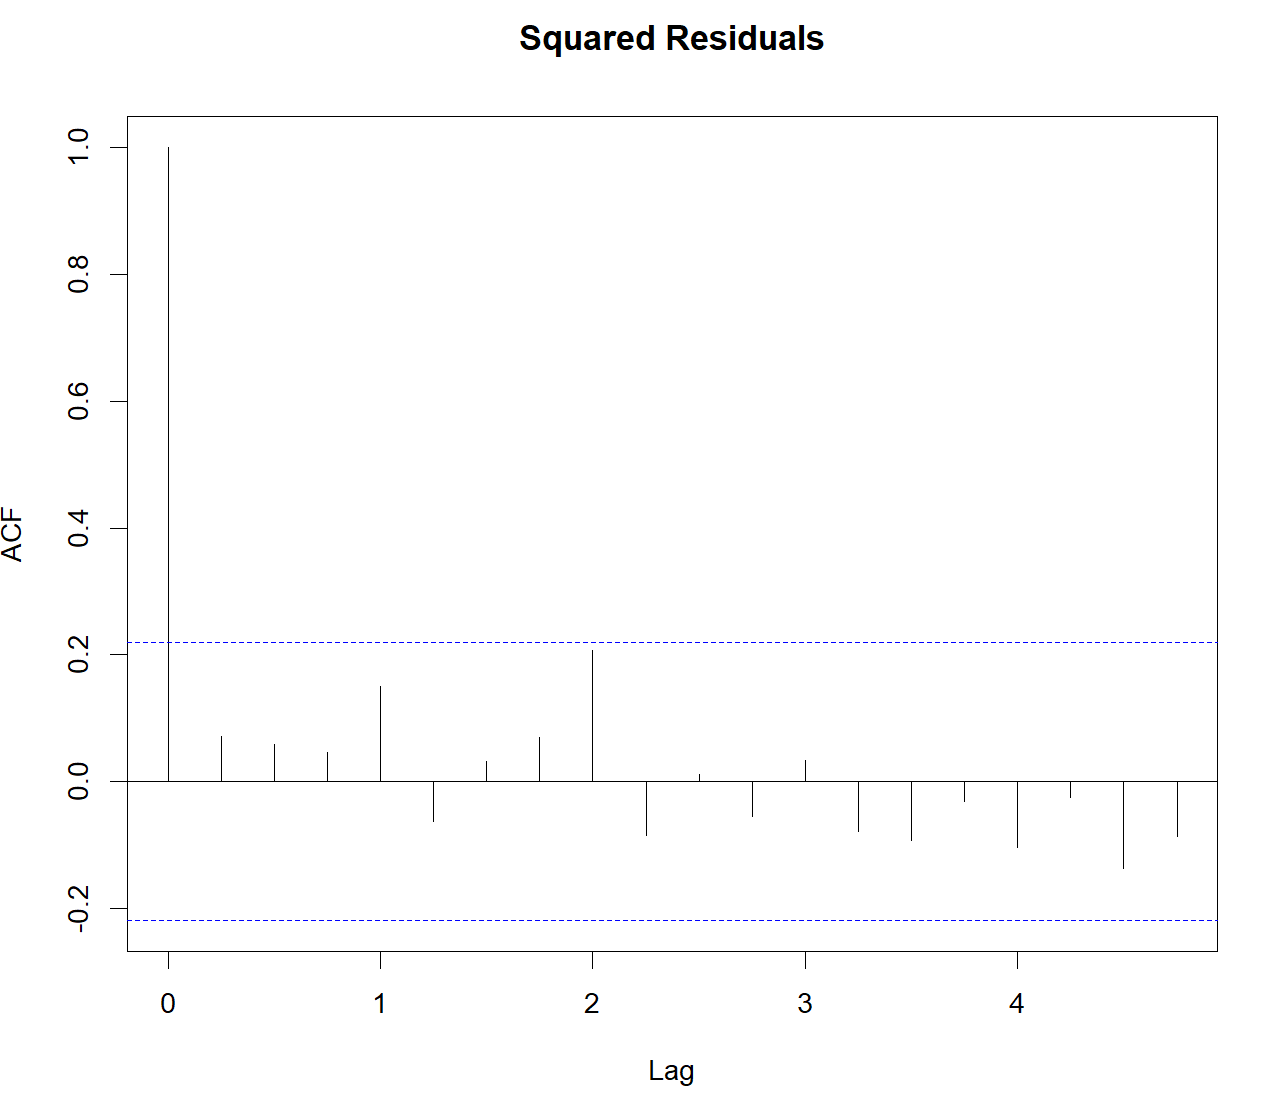
\includegraphics[width=0.6\linewidth]{fig/y1sq.png}
\end{figure}
The correlogram of the squared residuals shows no significant values, so there is no evidence of conditional heteroskedastic behaviour or volatility in the residual series, and an ARCH or GARCH model is not required.

\subsection{Holiday Series}
\begin{figure}[H]
    \centering
    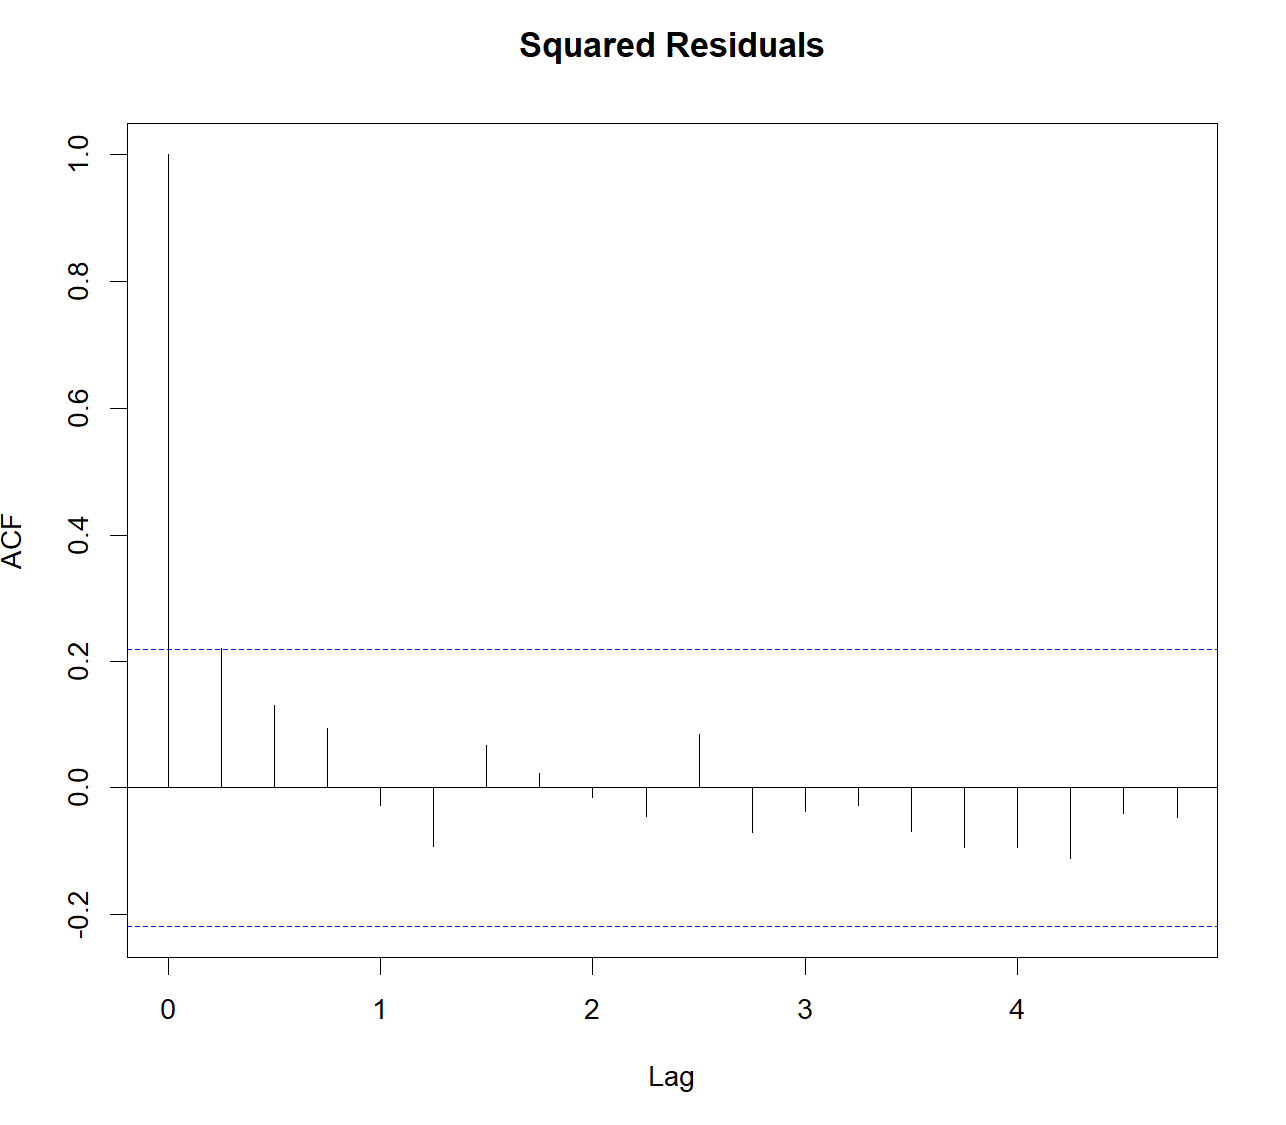
\includegraphics[width=0.6\linewidth]{fig/y2sq.png}
\end{figure}

The correlogram of the squared residuals does not show any significant spikes, which suggests that the residual variance remains relatively stable over time. There is no clear evidence of conditional heteroskedasticity or volatility clustering in the Holiday series. Therefore, a GARCH-type model is not necessary.

\subsection{Conclusion of the Two Series}

\noindent For the both Business and Holiday series shows that the squared residual correlograms do not show significant values. This suggests that both models have relatively stable residual variance and no strong volatility clustering. Hence, an ARCH or GARCH-type model is unnecessary for both series.



\vfill

\centering \textbf{\Large Scope of This Report}
\begin{table}[H]
\centering
\renewcommand{\arraystretch}{1.2}
\begin{tabular}{|p{13.5cm}|}
\hline
This was a two-person project. The Business series analysis in this report --
including the R implementation, model selection, interpretation, and report
writing for that series -- is my own work. The Holiday series analysis
follows the same structure and was conducted independently by a project
partner, reproduced here for completeness and comparison. \\
\hline
\end{tabular}
\end{table}
\end{document}